\cotefile{118}
\cotefile{118}
\scanpage{2}
Cohomology properties
of maps in $(\mathrm{Cat})$:

1) \unsure{Fibre-by-fibre}
properties

% archive foliation: 1

\scanpage{3}
% archive foliation: 2
\diagram{\begin{tikzcd}[column sep=small,row sep=large]
&&& F\cap C \arrow[dl,"F\cap C'"'] \arrow[dr,"F'\cap C"] &&& \\
&& F\cap\mathrm{Pr} \arrow[dl] \arrow[dr,"F'\cap\mathrm{Pr}"'] & \unsure{F'\cap C'} & \mathrm{Sm}\cap C \arrow[dl,"\mathrm{Sm}\cap C'"'] \arrow[dr] && \\
& F\cap S \arrow[dl] \arrow[dr,"F'\cap S"'] && \mathrm{Sm}\cap\mathrm{Pr} \arrow[dl] \arrow[dr] && S\cap C \arrow[dl,"S\cap C'"'] \arrow[dr] & \\
F \arrow[dr,"F'"'] && \mathrm{Sm}\cap S \arrow[dl] \arrow[dr] \arrow[dddd,dotted] && S\cap\mathrm{Pr} \arrow[dl] \arrow[dr] \arrow[dddd,dotted] && C \arrow[dl,"C'"'] \\
& \mathrm{Sm} && S \arrow[d] && \mathrm{Pr} & \\
&&& \mathrm{Spr}B \arrow[d] &&& \\
&&& \mathrm{Spr}F\cap\mathrm{Spr}C \arrow[dl] \arrow[dr] &&& \\
&& \mathrm{Spr}F && \mathrm{Spr}C &&
\end{tikzcd}}

\diagram{\begin{tikzcd}[column sep=small,row sep=large]
&&&&&& \mathrm{strh}\cap F\cap C \arrow[dl,dash] \arrow[dr] && \\
&&&&& \mathrm{strh}\cap F\cap\mathrm{strPr} \arrow[dl,dash] \arrow[dr,dash] && \mathrm{strh}\cap\mathrm{strSm}\cap C \arrow[dl,dash] \arrow[dr,dash] & \\
&& W\cap F\cap C \arrow[dl] \arrow[dr] \arrow[from=1-7,to=3-3,dash] && \mathrm{strh}\cap F \arrow[dr,dash] && \mathrm{strh}\cap\mathrm{strSm}\cap\mathrm{strPr} \arrow[dl,dash] \arrow[dr,dash] && \mathrm{strh}\cap C \arrow[dl,dash] \\
& W\cap F\cap\mathrm{Pr} \arrow[dl] \arrow[dr] && W\cap\mathrm{Sm}\cap C \arrow[dl] \arrow[dr] && \mathrm{strh}\cap\mathrm{strSm} \arrow[dr,dash] && \mathrm{strh}\cap\mathrm{strPr} \arrow[dl,dash] & \\
\begin{gathered}W\cap F\cap S\\=T\cap F\end{gathered} \arrow[dr] \arrow[from=3-5,to=5-1,dash,dashed] && W\cap\mathrm{Sm}\cap\mathrm{Pr} \arrow[dl] \arrow[dr] && \begin{gathered}W\cap S\cap C\\=T\cap C\end{gathered} \arrow[dl] \arrow[from=3-9,to=5-5,dash,dashed] && \mathrm{strh} \arrow[from=5-7,to=7-3,dash] && \\
& \begin{gathered}W\cap\mathrm{Sm}\cap S\\=T\cap\mathrm{Sm}\end{gathered} \arrow[dr] && \begin{gathered}W\cap S\cap\mathrm{Pr}\\=T\cap\mathrm{Pr}\end{gathered} \arrow[dl] &&&&& \\
&& \begin{gathered}W\cap S\\=T\cap S=\unsure{uW}\end{gathered} \arrow[d] &&&&&& \\
&& \begin{gathered}\mathrm{Bias}\\=W\cap\mathrm{Spr}B\end{gathered} \arrow[d] &&&&&& \\
&& \mathrm{As}\cap\mathrm{As}^{\circ} \arrow[dl] \arrow[dr] &&&&&& \\
& \begin{gathered}\mathrm{As}^{\circ}\\=W\cap\mathrm{Spr}F\end{gathered} \arrow[dr] && \mathrm{As}=W\cap\mathrm{Spr}C \arrow[dl] &&&&& \\
&& W &&&&&&
\end{tikzcd}}

\scanpage{4}
% archive foliation: 3
$3^{\circ})$ \uline{D. E. A.} :

\diagram{\begin{array}{lrr}
\text{\unsure{MM.} Auberson} & 748{,}80 & \\
\text{\phantom{MM. }Lefranc} & 374{,}40 & \\
\text{\phantom{MM. }Lemaire} & 748{,}80 & \\
\text{\phantom{MM. }Micali} & 1\ 497{,}60 & \\
\text{\phantom{MM. }Molino} & 1\ 497{,}60 & \\
\text{\phantom{MM. }Moreau} & 748{,}80 & \\ \cline{2-2}
& 5\ 616{,}00 & 5\ 616{,}00
\end{array}}

\uline{Contributions diverses} (placées pour raison comptable sous
la rubrique D.E.A.)

\diagram{\begin{array}{lcr}
\text{Reliquat 1980} & + & 977{,}71 \\
\text{Facture M. Lapscher} & + & 1\ 238{,}10 \\
\text{Facture Université Paul Valéry} & + & 1\ 750{,}00 \\
\text{Avoir Dawson} & + & 319{,}57 \\
\text{Facture M. Chein} & + & 144{,}90 \\
\text{Facture M. Lapscher} & + & \unsure{765{,}85|765{,}35} \\
\text{Facture M. Lapscher} & + & 212{,}45 \\
\text{Avoir Dawson (Fonctionnement - Autres crédits''} & + & 353{,}51 \\ \cline{3-3}
&& 6\ 262{,}09 \\[1em]
&& \boxed{11\ 878{,}09}
\end{array}}

$4^{\circ})$ \uline{Fonctionnement U.E.R. V} :

\diagram{\begin{array}{lcr}
\text{Reliquat 1980} & + & 920{,}23 \\
\text{Crédits Fonctionnement (Autres Crédits)} & + & 1\ 500{,}00 \\[1em]
\multicolumn{2}{r}{\text{Fonctionnement}} & \boxed{2\ 420{,}23} \\[2em]
\text{Crédits Fonctionnement (\unsure{HT}) Recherche} && \boxed{9\ 500{,}00}
\end{array}}

\scanpage{5}
% archive foliation: 4
\[
\boxed{\mathrm{Sm}\cap\mathrm{Pr}\subset S}
\]
\[
\boxed{\begin{gathered}WSC\cap\mathrm{Pr}\subset S\\ WSF\cap\mathrm{Sm}\subset S\end{gathered}}
\quad
\begin{gathered}
(\text{hence }WSC\cap\mathrm{Pr}=\inserted{\unsure{WSB\cap\deleted{\unsure{\mathrm{Pr}}}=}}(S\cap\mathrm{Pr}))\\
(\text{--- }WSF\cap\mathrm{Sm}=\unsure{S\cap\mathrm{Sm}})\\
\inserted{(WSB\cap\mathrm{Sm})}
\end{gathered}
\]
\margin{\diagram{\begin{tikzcd}[column sep=small]
S, \arrow[d,dash] & \mathrm{Pr}, \arrow[d,dash] & \mathrm{Sm} \arrow[d,dash] \\
\begin{gathered}\text{Serre map}\\\text{i.e. Hot-}\\\text{fibration}\end{gathered} & \text{proper} & \text{Smooth}
\end{tikzcd}}
$T=$ ``\unsure{univers.ly} in $W$''}

\margin{\deleted{$WSB\cap\mathrm{Sm}\unsure{\not\subset} \unsure{F}\ ?$}
\deleted{$(WSB\cap\mathrm{Pr}\unsure{\not\subset} C)$}

$WSB\neq WSF\cap WSC$ !

$WSC,WSB$ not stable under $S\cap C$ base ch.!
(And dually!) even if both are ``trivial''? $*$}

\margin{$C,\unsure{F|E}\unsure{\neq|\not\subset} WSF,WSC$ !
\deleted{$\unsure{C,F}$}
$\left[\begin{gathered}C\not\subset WSF\\F\not\subset WSC\end{gathered}\right]$

$C\cap WSF\not\subset S$ ?

$F\cap WSC\unsure{\not\subset}S$ ?}

\diagram{\begin{tikzcd}[column sep=small,row sep=large,
execute at end picture={\draw[dashed] (cutleft) -- (cuttop) -- (cutright);\draw[dashed] (cutlefttwo) -- (cuttoptwo) -- (cutrighttwo);}]
&&& \begin{gathered}\mathrm{def}\\B=F\cap C\end{gathered}\arrow[dl]\arrow[dr] &&& \\
&& F\cap\mathrm{Pr}\arrow[dl]\arrow[dr] & |[alias=cuttop]| {} & \mathrm{Sm}\cap C\arrow[dl]\arrow[dr] && \\
& F\cap S\arrow[dr]\arrow[dl,no head] && \mathrm{Sm}\cap\mathrm{Pr}\arrow[dl]\arrow[dr] && S\cap C\arrow[dl]\arrow[dr,no head] & \\
\underset{F\cap WSC}{\bullet}\arrow[d]\arrow[ddrr,gray] && \mathrm{Sm}\cap S\arrow[dl,no head]\arrow[ddr]\arrow[dddd,dotted,very thick] && S\cap\mathrm{Pr}\arrow[ddl]\arrow[dr,no head]\arrow[dddd,dotted,very thick] && \underset{WSF\cap C}{\bullet}\arrow[d]\arrow[ddll,gray] \\
|[draw,circle]| F\arrow[dr] & \underset{\mathrm{Sm}\cap WSC}{\bullet}\arrow[d] && |[alias=cuttoptwo]| {} && \underset{WSF\cap\mathrm{Pr}}{\bullet}\arrow[d] & |[draw,circle]| C\arrow[dl] \\
|[alias=cutleft]| {} & |[draw,circle]| \mathrm{Sm} && |[draw,circle]| S\arrow[d,"\unsure{\neq}"'] && |[draw,circle]| \mathrm{Pr} & |[alias=cutright]| {} \\
&&& |[draw,ellipse,dashed]| WSB\arrow[d] &&& \\
&& |[draw,ellipse,dashed]| \begin{gathered}\deleted{\unsure{\mathrm{Spr}F}}\\\inserted{WSF}\end{gathered}\arrow[ddr] & \begin{gathered}\deleted{\unsure{\mathrm{Spr}B}}\\WSF\cap WSC\end{gathered}\arrow[l]\arrow[r] & |[draw,ellipse,dashed]| \begin{gathered}\deleted{\unsure{\mathrm{Spr}C}}\\\inserted{WSC}\end{gathered}\arrow[ddl] && \\
& |[alias=cutlefttwo]| {} & \begin{gathered}(\deleted{\unsure{pre}}\text{ Serre pre-}\\\text{fibrations})\\\text{stable by}\\\text{proper b.ch.}\end{gathered} && \begin{gathered}(\deleted{\unsure{pre}}\text{ Serre}\\\text{precofibrations})\\\text{stable by}\\\text{smooth b.ch.}\end{gathered} & |[alias=cutrighttwo]| {} & \\
&&& \mathrm{Fl}(\mathrm{Cat}) &&&
\end{tikzcd}}
\margin{\unsure{str}}
\margin{stable under any base change

Squares cartesian}
\margin{\unsure{mon ch.|non ch.}

\unsure{tested by} $\Delta_1$ base ch.}

\margin{A Serre map is in $W$ iff \unsure{its} fibers are aspheric, i.e.
$S\cap W=S\cap T$
\inserted{and also iff it is univ. in $W$}}

\margin{Even if fibers are aspheric, the Serre condition cannot be tested by only taking base-changes $\Delta_1\to\unsure{Y}$ ?}

\margin{stable by intersection
\uline{except} $WSF\cap C$ and $\unsure{WCF}\cap\mathrm{Pr}$
and dually $F\cap WSC$, $\mathrm{Sm}\cap WSC$
and $WSF\cap WSC$}

\margin{$*$ i.e. find $f:X\to Y$, $g:Y'\to Y$
with $f\in W\cap WSB$ (i.e. $f$ tot. asph)
\deleted{$W$} and $g\in T\cap C$ (cofibration with trivial fibers) s.th.
$f':X'\longrightarrow Y'$ is not in $WSE$
(say $Y'$ with final element $e$ and $y'\in\mathrm{Ob}\,Y'$ s.th.
$X'_{/y'}\to X'_{/e}$ not a Weak equiv. ?}

\diagram{\begin{tikzcd}[column sep=small,row sep=large,
execute at end picture={\draw[dashed] (lowcutleft) -- (lowcuttop) -- (lowcutright);\draw[dashed] (lowcutlefttwo) -- (lowcuttoptwo) -- (lowcutrighttwo);}]
&& \unsure{\overline{W}}\cap F\cap C\arrow[dl,"\mathrm{str}"']\arrow[dr] && \\
& \unsure{\overline{W}}\cap F\cap\mathrm{Pr}\arrow[dl,"\mathrm{str}"']\arrow[dr] & |[alias=lowcuttop]| {} & W\cap\mathrm{Sm}\cap C\arrow[dl]\arrow[dr] & \\
\begin{gathered}W\cap F\cap S\\\deleted{\unsure{W}}=T\cap F\end{gathered}\arrow[dr] && W\cap\mathrm{Sm}\cap\mathrm{Pr}\arrow[dl]\arrow[dr] && \begin{gathered}W\cap S\cap C\\=T\cap C\end{gathered}\arrow[dl] \\
|[alias=lowcutleft]| {} & \begin{gathered}W\cap\mathrm{Sm}\cap S\\=T\cap\mathrm{Sm}\end{gathered}\arrow[dr] & |[alias=lowcuttoptwo]| {} & \begin{gathered}W\cap S\cap\mathrm{Pr}\\=T\cap\mathrm{Pr}\end{gathered}\arrow[dl] & |[alias=lowcutright]| {} \\
&& |[draw,ellipse,double]| \begin{gathered}W\cap S\\=T\cap S=\unsure{uW}\end{gathered}\arrow[d,"\mathrm{str}"] && \\
|[alias=lowcutlefttwo]| {} && |[draw,ellipse,dashed]| \begin{gathered}\mathrm{Tot\ As}\\=W\cap WSB\end{gathered}\arrow[dl,"\mathrm{str}"']\arrow[dr] && |[alias=lowcutrighttwo]| {} \\
& |[draw,ellipse,double]| \begin{gathered}\mathrm{As}^{\circ}\\\deleted{\unsure{\mathrm{As}}}\\=W\cap WSF\end{gathered}\arrow[dr,"\mathrm{str}"'] && |[draw,ellipse,double]| \begin{gathered}\mathrm{As}\deleted{\unsure{^{\circ}}}\\=W\cap WSC\end{gathered}\arrow[dl] & \\
& \begin{gathered}(\text{stable by}\\\text{proper b.ch.})\end{gathered} & W & \begin{gathered}(\text{stable by}\\\text{smooth b.ch.})\end{gathered} & \\
&& \begin{gathered}(\text{stable by}\\S\text{ base ch.})\end{gathered} &&
\end{tikzcd}}
\margin{Stable under any base change

Squares cartesian}
\margin{this square $\longrightarrow$
non cartesian?}
\margin{stable by intersection except $\mathrm{As}\cap\mathrm{As}^{\circ}$}

\scanpage{6}
% archive foliation: 5
% Landscape sheet; the writing is read after a quarter-turn counterclockwise.
\diagram{\begin{array}{lc@{\qquad}lc}
\multicolumn{2}{l}{\text{Séminaire de Mécanique}} & \multicolumn{2}{l}{\text{Séminaire de Géométrie Différentielle}}\\[1em]
\cline{1-2}\cline{3-4}
\begin{array}{l|l}\text{---}\qquad & \qquad\qquad\\[12em]&\end{array}
&&
\begin{array}{rl|l}
1217{,}00 & \text{M. Kumpera} & \qquad\qquad\\
1146{,}10 & \text{M Van Est} & \\ \cline{1-1}
2363{,}10 & \text{Total} & \\[10em]
&&
\end{array}
& \\
\cline{1-2}\cline{3-4}
\end{array}}

\scanpage{7}
% archive foliation: 6
% Landscape sheet; the writing is read after a quarter-turn counterclockwise.
\diagram{\begin{array}{lc@{\qquad}lc}
\multicolumn{2}{l}{\text{Séminaire d'Analyse Fonctionnelle}} & \multicolumn{2}{l}{\text{Séminaire d'Analyse Convexe}}\\[1em]
\cline{1-2}\cline{3-4}
\begin{array}{l|l}\text{---}\qquad & \qquad\qquad\\[12em]&\end{array}
&&
\begin{array}{rl|l}
285{,}00 & \text{M. Gossez} & \qquad\qquad\\
709{,}50 & \text{M. Klei} & \\
1\ 004{,}50 & \text{M. \unsure{Pallu de la Barrière}} & \\
565{,}50 & \text{M. Singer} & \\ \cline{1-1}
2\ 564{,}50 & \text{Total} & \\[8em]
&&
\end{array}
& \\
\cline{1-2}\cline{3-4}
\end{array}}

\scanpage{8}
% archive foliation: 7
\[
\unsure{TF|T\cap F}\quad\deleted{\unsure{T}}\quad\unsure{\not\subset}T\deleted{\unsure{F}}\unsure{'|!}
\]
\diagram{\begin{tikzcd}
X\arrow[d]\arrow[d,bend right=25] & \text{\uline{strict \unsure{homotopism}}} \\
Y &
\end{tikzcd}}

\scanpage{9}
% archive foliation: 8
$f:X\unsure{\to}Y$

\diagram{\begin{tikzcd}[column sep=small,row sep=large]
\text{\textcircled{\unsure{0}}}\quad f\in C\arrow[r,Leftrightarrow] & \begin{gathered}X_b\to X_{/b}\text{ : adj. à gauche}\end{gathered}\arrow[d,Leftrightarrow] & f\in F\arrow[r,Leftrightarrow] & {}\arrow[d,Leftrightarrow] \\
& \begin{gathered}{}_{a}\backslash X\to{}_{b}\backslash\unsure{X|Y}\text{ à fibres avec}\\\text{objet initial}\end{gathered}\arrow[d,Leftrightarrow] && {}\arrow[d,Leftrightarrow] \\
& \begin{gathered}\text{La catégorie des relèv. d'une}\\\text{flèche }b\to b',\text{ de source}\\\text{donnée }a\in X_b,\text{ a objet initial}\end{gathered} && {}
\end{tikzcd}}

\diagram{\begin{tikzcd}[column sep=small,row sep=large]
\text{\textcircled{2}}\quad f\in\mathrm{Pr}\arrow[r,Leftrightarrow] & \begin{gathered}(\unsure{X_b}\to X_{/b})\text{ \unsure{strong} \inserted{$\leftarrow$} équiv ie coasph.}\\\text{i.e. }\in\mathrm{As}^{\circ}\end{gathered}\arrow[d,Leftrightarrow] & f\in\mathrm{Sm}\arrow[r,Leftrightarrow] & {}\arrow[d,Leftrightarrow] \\
& \begin{gathered}{}_{a}\backslash X\to{}_{b}\backslash Y\text{ à fibres asph.}\\\deleted{\unsure{{}_{a}\backslash X\to{}_{b}\backslash Y}}\quad({}_{a}\backslash X\to{}_{b}\backslash Y)\in S\quad\deleted{\unsure{\Longleftrightarrow({}_{a}X\to{}_{a}X)}}\end{gathered}\arrow[d,Leftrightarrow] && {}\arrow[d,Leftrightarrow] \\
& \begin{gathered}\text{La cat. des rel. d'une flèche }b\to b',\\\text{de source donnée }a\in\mathrm{Ob}\,\unsure{X_b},\text{ est asph.}\end{gathered}\arrow[d,Leftrightarrow] && {}\arrow[d,Leftrightarrow] \\
& \begin{gathered}R^i f_*\text{ commute }\deleted{\unsure{\Longrightarrow}}\text{ aux chgt de base}\\\text{quelc.}\end{gathered} && \begin{gathered}\text{\unsure{Le changt} de base par }f\\\text{commute à }R^i g_*\end{gathered} \\
& \left[\overset{?}{\Longrightarrow}\text{ base change by }f\text{ preserves \unsure{strong} équiv}\right] && \left[\overset{?}{\Longleftarrow}\quad\right]
\end{tikzcd}}
\margin{\diagram{\begin{tikzcd}
{}\arrow[d,Rightarrow]\\
\begin{gathered}({}_{a}X\to{}_{b}Y\text{ is}\\\text{proper}\\\text{with \unsure{trivial}}\\\text{fibers})\end{gathered}
\end{tikzcd}}}

\[
\text{\textcircled{1}}\quad f\in S\Longleftrightarrow
\forall\ g:Y''\to Y',\text{ sur }Y,\text{ si }g\in W,\text{ alors }(g\times_Y X:X''\to X')\in W.
\]

\diagram{\begin{array}{ccc}
\boxed{\left\{\begin{gathered}F\Longrightarrow\mathrm{Sm}\\C\Longrightarrow\mathrm{Pr}\end{gathered}\right.}
& \begin{gathered}\boxed{\mathrm{Sm}\cap\mathrm{Pr}\Longrightarrow S}\\\boxed{T\cap\mathrm{Pr}\subset S,\ T\cap\mathrm{Sm}\subset S}\end{gathered}
& \begin{gathered}\left\{\begin{gathered}C=F^{\circ},\ \deleted{\unsure{C\in C^{\circ}}}\\F=C^{\circ}\end{gathered}\right.\quad S=S^{\circ}\quad
\left\{\begin{gathered}\mathrm{Sm}=\mathrm{Pr}^{\circ}\\\mathrm{Pr}=\mathrm{Sm}^{\circ}\end{gathered}\right.\end{gathered}
\end{array}}

\diagram{\begin{tikzcd}[column sep=small,row sep=large]
\text{\textcircled{3}}\quad f\in WSC\arrow[r,Leftrightarrow] & \forall b\to b'\text{ dans }Y,\ (X_{/b}\to X_{/b'})\in W\quad\text{\textcircled{a}}\arrow[d,Leftrightarrow] & f\in WSF\arrow[r,Leftrightarrow] & {}\arrow[d,Leftrightarrow] \\
& \left\{\begin{gathered}\forall\ Y''\xrightarrow{u}Y'\text{ sur }Y,\ Y''\text{ et }Y'\ \deleted{\text{\unsure{fibrés}}}\inserted{\text{cofibrés}}\text{ in }C,\\\text{si }u\in W,\text{ alors }(g\times_Y X:X''\to X')\in W\end{gathered}\right.\quad\text{\textcircled{b}}\arrow[d,Leftrightarrow]\arrow[l,Rightarrow] && {}\arrow[d,Leftrightarrow] \\
& \deleted{\unsure{\Longleftrightarrow}}\quad(\mathrm{Cofib}(X/Y)\to Y)\ \deleted{\unsure{\in W}}\in S\ \unsure{\in}\quad\text{\textcircled{a$'$}} && (\mathrm{Fib}(X/Y)\to Y)
\end{tikzcd}}
\margin{$\Longleftarrow$ $R^i f_*(\unsure{c^t})$ loc \unsure{constants}}

\uline{stable par chgt de base par \deleted{fibrations}\inserted{\unsure{fonct.} lisses}},
(mais non par $g\in S$ ?)
\margin{stable par chgt de base \uline{propres}}

\[
\boxed{WSC\cap\mathrm{Pr}\subset S}\qquad
\boxed{WSF\cap\mathrm{Sm}\subset S}
\]

\textcircled{3bis} $f\in WSB\deleted{\unsure{F}}\underset{\mathrm{déf}}{\Longleftrightarrow}$
\inserted{$\deleted{\unsure{\in}}\unsure{WSF}\Longrightarrow$}
pour
\diagram{\begin{tikzcd}
b'_0\arrow[r]\arrow[rrr,bend right=25,"u'"'] & b_0\arrow[r,"u"] & b_1\arrow[r] & b'_1
\end{tikzcd}}
dans $Y$,
\diagram{\begin{tikzcd}[column sep=large]
|[draw,ellipse]| {}_{b_0}\backslash X_{/b_1}\arrow[r]\arrow[d,dash] & |[draw,ellipse]| {}_{b'_0}\backslash X_{/b'_1}\arrow[ddl,dash] & \text{est }\in W,\text{ i.e. l'équiv.} \\
\inserted{X[u]} & \unsure{\text{for}} & \\
\inserted{X[u']} &&
\end{tikzcd}}
\[
{}_{b_0}\backslash Y_{/b_1}\to{}_{b'_0}\backslash Y_{/b'_1}
\]
\deleted{\unsure{dans}} $Y$ est \unsure{transformée} en équiv. faible par $\unsure{X|Y}\times(?)$.
\[
\Updownarrow\quad\forall b\to b'\text{ dans }Y,\quad
{}_{b'}\backslash X\to{}_{b}\backslash X\text{ est }\in W\text{ loc. sur }Y.
\]
\[
\deleted{\text{et}}\quad\forall b\to b'\text{ dans }Y,\quad
X_{/b}\to X_{/b'}\text{ est }\in W\text{ \unsure{coloc.} sur }Y
\]

\scanpage{10}
% archive foliation: 9
UNIVERSITE DES SCIENCES ET TECHNIQUES
DU LANGUEDOC

MATHEMATIQUES

Place E.-Bataillon

34060 MONTPELLIER CEDEX

\unsure{M. Grothendieck}

\uline{FERMETURE ``SPÉCIAL QUICK'' POUR ENVOI NON CLOS}

Peut être ouvert pour contrôle par le Service Postal

Pour ouvrir, tirer sur le rabat - Refermer par simple pression

(Note P. O. A 3 du \unsure{14.6.73|14.6.63} - \unsure{B. O. 190} \unsure{P. C. 23|P. 6. 23}

\scanpage{11}
\uline{\unsure{Coh. prop. of maps in Cat}}

2) Immersions fermées et ouvertes

\uline{Propriétés cohomologiques}

\margin{not cofib. nor fib. (i.e. not closed imm nor open imm)}

\diagram{\begin{tikzcd}[column sep=large]
Y & \mathrm{Fib}(f) \arrow[l,"\unsure{f^b|f^\flat}","\text{fibration}"'] \arrow[r,bend right=35,"\rho_f"'] & X \arrow[l,"\unsure{\eta_f|H_f}\ \text{mono}"']
\end{tikzcd}}

(Fibers ${}_{b}\backslash X$ discretely cofibered /$X$)

\uline{but not yet} \uline{Serre}

(Serre cofibering) retraction

[fibers $Y_{/b}$ discr. fibered over $Y$]

\diagram{\begin{tikzcd}[column sep=large]
Y & \mathrm{Cofib}(f) \arrow[l,"\unsure{f^{b'}|f^{\flat\prime}}","\text{cofibration}"'] \arrow[r,bend right=35,"\rho'_f"'] & X \arrow[l,"\unsure{\eta'_f|H'_f}\ \text{mono}"']
\end{tikzcd}}

(fibers $X_{/b}$ discretely fibered /$X$)

\uline{but not yet Serre}

Serre \unsure{fibering} retraction

(fibers ${}_{b}\backslash Y$ discr. cofibered over $Y$)

but not

\figure{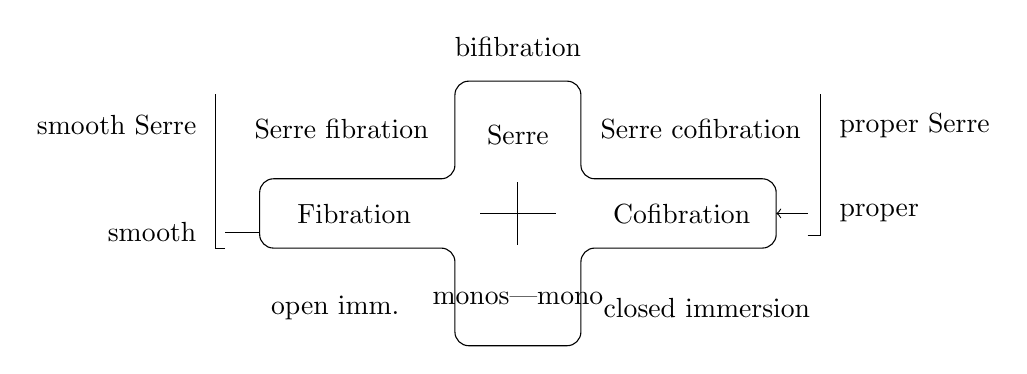
\begin{tikzpicture}[x=0.8cm,y=0.8cm]
\draw[rounded corners=5pt] (-1,2.1)--(1,2.1)--(1,.55)--(4.1,.55)--(4.1,-.55)--(1,-.55)--(1,-2.1)--(-1,-2.1)--(-1,-.55)--(-4.1,-.55)--(-4.1,.55)--(-1,.55)--cycle;
\draw (-.6,0)--(.6,0) (0,-.5)--(0,.5);
\node at (0,1.25) {Serre};
\node at (0,-1.35) {\unsure{monos|mono}};
\node at (-2.6,0) {Fibration};
\node at (2.6,0) {Cofibration};
\node at (0,2.65) {bifibration};
\node at (-2.8,1.35) {Serre fibration};
\node at (2.9,1.35) {Serre cofibration};
\node at (-2.9,-1.5) {open imm.};
\node at (3,-1.5) {closed immersion};
\draw (-4.1,-.3)--(-4.65,-.3) (-4.65,-.55)--(-4.8,-.55)--(-4.8,1.9);
\node[anchor=east] at (-4.95,1.4) {smooth Serre};
\node[anchor=east] at (-4.95,-.3) {smooth};
\draw[<-] (4.1,0)--(4.6,0);
\draw (4.6,-.35)--(4.8,-.35)--(4.8,1.9);
\node[anchor=west] at (4.95,1.4) {proper Serre};
\node[anchor=west] at (4.95,0) {proper};
\end{tikzpicture}}

\diagram{\begin{tikzcd}[column sep=large]
Y \arrow[r,hook,"\unsure{f^b|f^\flat}","\text{open imm}"'] & C(f) \arrow[r,"\lambda_f^{(\mathrm{op})}"] & X \arrow[l,bend left=35,"\sigma_f","\text{closed section}"']
\end{tikzcd}}

\diagram{\begin{tikzcd}[column sep=large]
Y \arrow[r,hook,"\unsure{f^{b'}|f^{\flat\prime}}\ \text{closed}","\text{imm}"'] & C'(f) \arrow[r,"\lambda'_f"] & X \arrow[l,bend left=35,"\sigma'_f","\text{open section}"']
\end{tikzcd}}

\diagram{\begin{tikzcd}[column sep=large]
Y \arrow[r,hook,"i_Y","\text{open imm}"'] & C(Y) \arrow[r,"\varepsilon_Y"] & e \arrow[l,bend left=35,"\text{closed section}"']
\end{tikzcd}}

($e$ \inserted{strict} final object)

\diagram{\begin{tikzcd}[column sep=large]
Y \arrow[r,hook,"i'_Y","\text{closed imm}"'] & C'(Y) \arrow[r,"\varepsilon'_Y"] & e \arrow[l,bend left=35,"\text{open section}"']
\end{tikzcd}}

($e$ strict initial object)

\[
C'(f)^\circ=C(f^\circ)\quad\text{i.e.}\quad C'(f)=C(f^\circ)^\circ
\]
\[
C'(Y)^\circ=C(Y^\circ)\quad\text{i.e.}\quad C'(Y)=C(Y^\circ)^\circ
\]
% archive foliation: 10

\scanpage{12}
\diagram{\begin{tikzcd}[column sep=large,row sep=large]
Y & \mathrm{Fl}(Y) \arrow[l] \arrow[d] & \mathrm{Fib}(f) \arrow[l] \arrow[ll,bend right=30,"\unsure{f^b|f^\flat}"'] \arrow[d,"\rho_f"]\\
 & \unsure{Y|Y'} \arrow[u,dashed,bend right=30] & X \arrow[l,"f"'] \arrow[u,dashed,bend right=45,"\unsure{\eta_f|H_f}"']
\end{tikzcd}}

\diagram{\begin{tikzcd}[column sep=large]
Y & \mathrm{Fib}(f) \arrow[l,"\unsure{f^b|f^\flat}","\text{fibration}"'] \arrow[r,bend right=30,"\rho_f"'] & X \arrow[l,"\unsure{\eta_f|H_f}\ \text{mono}"']
\end{tikzcd}}

(fibers ${}_{b}\backslash X$ discretely cofibered over $X$)

\uline{but not yet Serre}

trivial Serre \unsure{cofibering} retraction

(fibers $Y_{/b}$ discr. fibred over $Y$)

and homotopism

\figure{\begin{tikzpicture}[x=.8cm,y=.8cm]
\draw[rounded corners=12pt] (-.7,3.1)--(.7,3.1)--(.7,.5)--(4.6,.5)--(4.6,-.5)--(.7,-.5)--(.7,-2.7)--(-.7,-2.7)--(-.7,-.5)--(-4.6,-.5)--(-4.6,.5)--(-.7,.5)--cycle;
\draw[line width=1.6pt] (-.45,0)--(.45,0) (0,-.45)--(0,.45);
\node at (0,2.65) {Serre};
\node[align=center] at (0,1.05) {$[\mathrm{Serre}\cap W$\\$=\text{triv.Serre}]$};
\draw[->] (0,1.5)--(0,2.35);
\node at (-2.65,0) {smooth $\longleftrightarrow$ \uline{fibration}};
\node at (2.65,0) {\uline{cofibration} $\longleftrightarrow$ proper};
\node[align=center] at (0,-1) {mono\\\deleted{\unsure{fibered} \unsure{discrete}}};
\draw[->] (0,-1.45)--(0,-2.05);
\node at (0,-2.35) {discrete};
\draw (-4.6,1.7)--(-1,1.7) (-3.1,.7)--(-3.1,2.8);
\node at (-4,2.35) {Smooth Serre};
\node at (-1.95,2.35) {Serre fibration};
\node at (-4,1.05) {trivial smooth};
\node at (-1.95,1.05) {trivial fibration};
\draw (1,1.7)--(4.9,1.7) (2.9,.7)--(2.9,2.8);
\node at (1.8,2.35) {Serre cofibration};
\node at (4,2.35) {Serre proper};
\node at (1.8,1.05) {trivial cofibration};
\node at (4,1.05) {trivial proper};
\node[anchor=east,align=right] at (-.85,-1.2) {$\left.\begin{gathered}
\text{open immersions}\longleftrightarrow X^\circ\xrightarrow{\varphi}\Delta^1=[0\longrightarrow1]\\
\longleftrightarrow\unsure{\mathrm{crib}}(X)\\
Y=\varphi^{-1}(\{1\})=\psi^{-1}(\{0\})=X_0
\end{gathered}\right\}$};
\node[anchor=east] at (-.85,-2.5) {$\left.\text{discrete fibrations}\longleftrightarrow\widehat X,\text{i.e. }X^\circ\longrightarrow(\mathrm{Sets})\right\}$};
\node[anchor=west,align=left] at (.85,-1.2) {$\left\{\begin{gathered}
\text{Closed immersions}\longleftrightarrow X\xrightarrow{\varphi}\Delta^1=\left[\overset{\substack{0\\\Vert}}{\varnothing}\to\overset{\substack{1\\\Vert}}{\{\varnothing\}}\right]\\
=\hspace{3cm}\Longleftrightarrow\mathrm{Cocrib}(X)\\
Y=\varphi^{-1}(\{1\})=X_1
\end{gathered}\right.$};
\node[anchor=west] at (.85,-2.5) {$\left\{\text{discrete cofibration}\Longleftrightarrow\check X,\text{i.e. }X\longrightarrow(\mathrm{Sets})\right.$};
\end{tikzpicture}}

\margin{(où $\psi:X\xrightarrow{\varphi^\circ}\Delta_1^\circ\xrightarrow[\sim]{\mathrm{can.}}\Delta_1$)}

\diagram{\begin{tikzcd}[column sep=large]
Y \arrow[r,hook,"f^\sharp","\text{open imm}"'] & C(f) \arrow[r,"\lambda_f\ \text{epi}"] & X \arrow[l,bend left=35,"\sigma_f","\substack{\text{closed section}\\\text{and \uline{homotopism}}}"']
\end{tikzcd}}

\diagram{\begin{tikzcd}[column sep=large]
Y \arrow[r,hook,"f^{\sharp\prime}","\text{closed imm.}"'] & C'(f) \arrow[r,"\lambda'_f"] & X \arrow[l,bend left=35,"\sigma'_f","\substack{\text{open section}\\\text{\uline{and homotopism}}}"']
\end{tikzcd}}

\margin{$\text{discret}\cap\mathrm{Serre}\;(=\text{étale covering})\subset\text{smooth}\cap\text{proper}\unsure{\subset}\overset{\unsure{\text{étale}}}{\mathrm{Serre}}$

\deleted{$\text{mono}\cap\mathrm{Serre}$} $=$ \deleted{open} closed imm $=$ $\overset{\unsure{=\mathrm{Serre}}}{\text{direct summand}}$

$\unsure{\text{discret}}\cap\unsure{\text{triv.Serre}|\text{strictSerre}}=\mathrm{iso}$

\uline{NB} $\text{proper}\cap\text{discret}\Rightarrow\text{cofib}$, $\text{smooth}\cap\text{discret}\Rightarrow\text{fibration}$

but does not imply mono, and $\text{proper}\cap\text{free}$ does not imply cofibration \inserted{nor trivial}, $\text{smooth}\cap\text{free}$ not imply fibration \inserted{nor trivial}}
% archive foliation: 11

\scanpage{14}
\diagram{\begin{array}{l|l}
f^\sharp\in\text{fibration}\cap\text{mono}&\unsure{f^b|f^\flat}\in\text{fibration (not \uuline{yet Serre})}\\\hline
\sigma_f\in\text{cofibration}\cap\text{mono}\cap\mathrm{tr}&\rho_f\in\text{cofibration}\cap\mathrm{Serre}\cap\mathrm{tr}\\\hline
\lambda_f\unsure{\notin}\;\big|\;\begin{gathered}\text{not a fibration or cofibration}\\\text{nor Serre, but trivial}\\\text{fibers (with final}\\\text{object}\end{gathered}&
\unsure{\eta_f|H_f}\unsure{\notin}\;\big|\;\begin{gathered}\text{not a fibration nor cofibration}\\\text{nor Serre ?}\end{gathered}
\end{array}}

\margin{NB $\text{proper discret}\Rightarrow\text{cofib}$

$\text{smooth discret}\Rightarrow\text{fibration}$

$\left[\begin{gathered}\text{but proper Serre}\not\Rightarrow\text{cofib}\\\text{smooth Serre}\not\Rightarrow\text{fib}\end{gathered}\right]$}

\diagram{\begin{tikzcd}
(Y\longrightarrow X) \arrow[r] & X & & Y\\
 & Y_x \arrow[r] & \deleted{\unsure{X|x}}\\
0 \arrow[r] & 1
\end{tikzcd}}

$(\lambda_f,\sigma_f)$ adjoint ?

$(\unsure{\eta_f|H_f},\rho_f)$ adjoint

\diagram{\begin{tikzcd}[execute at end picture={\draw (current bounding box.center) ellipse [x radius=3.7cm,y radius=1.15cm];}]
X\arrow[r]&\text{Cofiber of }f^\sharp\;?\\
Y\arrow[r]&\text{Cofiber of }\sigma_f\;?
\end{tikzcd}}

\figure{\begin{tikzpicture}[x=.9cm,y=.9cm]
\draw[line width=1.3pt] (-.35,0)--(.35,0) (0,-.35)--(0,.35);
\node at (0,.7) {Serre};
\node at (0,1.8) {bifibration};
\draw[->] (0,1)--(0,1.5);
\node at (-2.35,0) {smooth $\unsure{\subset}$ fibration};
\node at (2.3,0) {proper $\supset$ co- \unsure{proper}};
\draw (-5.5,0)--(-4,0) (4.1,0)--(5.5,0);
\node at (0,-.9) {discrete};
\node[gray] at (0,-1.5) {\unsure{mono}};
\draw[->] (0,-1.1)--(0,-1.65);
\node at (0,-2) {mono};
\node[anchor=east,align=left] at (-.5,-1) {$\left.\begin{gathered}\text{discrete fibration}\\\widehat X\text{ i.e. }X^\circ\longrightarrow(\mathrm{Sets})\end{gathered}\right\}$};
\node[anchor=west,align=left] at (.5,-1) {$\left\{\begin{gathered}\text{discrete cofibration}\\\check X\text{ i.e. }X\longrightarrow(\mathrm{Sets})\end{gathered}\right.$};
\node[anchor=east,align=left] at (-.5,-3.1) {$\left.\begin{gathered}
X^\circ\longrightarrow\left[\overset{\substack{0\\\Vert}}{\varnothing},\overset{\substack{1\\\Vert}}{\{\varnothing\}}\right]=\Delta_1\\
Y=\varphi^{-1}(\{1\})=\unsure{\psi|\varphi}^{-1}(\{0\})\\
(\psi:X\xrightarrow{\varphi^\circ}\Delta_1^\circ\simeq\Delta_1\\
\text{open immersion}
\end{gathered}\right\}$};
\node[anchor=west,align=left] at (.5,-3) {$\left\{\begin{gathered}
X\xrightarrow{\varphi'}[\varnothing,\{\varnothing\}]=\unsure{\Delta^1_1|\Delta_1}:\;[0\longrightarrow1]\\
Y=\varphi'^{-1}(\{1\})\\
\text{closed immersion}
\end{gathered}\right.$};
\end{tikzpicture}}
% archive foliation: 13

\scanpage{15}
Après \unsure{l'axiome} d'asphéricité : \unsure{corps de} \unsure{Loc 4|Loc 1}, Loc 2, Loc 3,

(\uline{Loc} 1 sous forme faible

a) iso dans $\underline W$

b) si deux parmi $g,f,gf$ dans $\underline W$, le 3e l'est

c) $gf=\mathrm{id}$ et $fg\in\underline W\Rightarrow f,g\in\underline W$)

\textcircled{0} Axiomes Loc mettons au net \unsure{les props} \unsure{constructions} fibs et cofib.

\textcircled{1} \uline{Dualité} (y compris $\underline W=\underline W^\circ$)

\margin{\textcircled{2} Commentaire sur fibrations cofibrations imm. ouvertes, '' fermées Cylindres Cônes \ldots}

\deleted{\textcircled{2}}\inserted{\textcircled{3}} \unsure{a)} Soit des
\diagram{\begin{tikzcd}[column sep=small,row sep=small]
\unsure{\displaystyle\int}\!Y\arrow[r]\arrow[d]&X_0\\X_1&
\end{tikzcd}}

\diagram{\begin{tikzcd}[column sep=large,row sep=large]
Y\arrow[r,"f_0"]\arrow[d,"f_1"']\arrow[dr,"\deleted{\unsure{\beta}}" description]&X_0\arrow[d,"\alpha_1"]&\\
X_1\arrow[r,"\deleted{\unsure{q_1}}\ \unsure{\lambda_g}","\unsure{\alpha_0}\ \deleted{\unsure{q_0}}"']&\Sigma\arrow[dr]&\\
&&X_0\amalg_Y X_1
\end{tikzcd}}

et passage \unsure{:|à} la limite

\deleted{Si $f_0$ iso, $q_0$ homotopisme}

a) \uline{Fonctorialité} si $u_Y,u_{X_0},u_{X_1}\in\underline W$, alors $(\Sigma\to\Sigma')\in\underline W$

b) Si $f_0$ iso, alors $\unsure{\alpha_0}$ homotopisme (it. $f_1,\alpha_1$

c) Si $f_0\in\underline W$, alors $\unsure{\alpha_0}\in\underline W$ (it. $f_1,\alpha_1$)

\deleted{\textcircled{\unsure{3}}}\inserted{\textcircled{4}} \deleted{\textcircled{\unsure{a}}} \uline{Thm} du

\margin{``de la somme amalgamée'' (dans (Cat))}

\diagram{\begin{tikzcd}
Y\arrow[r,"f_0"]\arrow[d,"f_1"']&X_0\arrow[d,"q_1"]\\
X_1\arrow[r,"q_0"']\arrow[ur,phantom,"\mathrm{cart}" description]&X
\end{tikzcd}}

avec $q_0,q_1$ cofibrations (resp. fibrations)

Supposons que $\forall x\in X$, $X_{0x}$ \unsure{ou} $X_{1x}$ sont \deleted{\unsure{quasi}} \inserted{$\underline W$-}asphériques. Alors

\diagram{\begin{tikzcd}
\displaystyle\int\begin{gathered}Y\longrightarrow X_0\\\downarrow\hspace{1.6cm}\\X_1\hspace{1.6cm}\end{gathered}\arrow[r]&X
\end{tikzcd}}

cofib (resp. fib) à fibres triviales, donc $U\underline W$.

\margin{\uline{NB} Si on suppose \deleted{\unsure{en}} que $\forall a\in X$,
\deleted{$\unsure{X_{0a}}$ \unsure{ou} $\unsure{X_{1a}}$ \unsure{soit}}\inserted{tels que l'une des}
\deleted{\unsure{cat. ponctuelles}, \unsure{l'une des}}
\deleted{\unsure{cat.}} $X_{0a},X_{1a}$ soit $\varnothing$, l'autre soit isom. à $\Delta_0$, alors ce diagramme est cocartésien, et le reste par tt chgt de base (\unsure{ci voir près})}

\uline{Cor.} Si $f_0\in\underline W$, alors $q_0\in\underline W$

Si $f_1\in\underline W$, alors $q_1\in\underline W$

Cas
\diagram{\begin{tikzcd}
Y\arrow[r,hook,"i"]\arrow[d,"f"']&X\arrow[d,"g"]\\
Y'\arrow[r,dash,"i'"']&X'=X\amalg_Y Y'
\end{tikzcd}}

$i$ imm. ouverte ou fermée

\uline{Question} --- si $f$ \unsure{asphérique|cofibré}, il n'en résulte pas que $g$ le soit, et si $f\in\underline W$, il est possible qu'on n'ait pas $g\in\underline W$,

[mais j'ignore si $i\in\underline W$ implique $i'\in\underline W$]

\deleted{\textcircled{\unsure{4}}}\inserted{\textcircled{c}} \uline{Application} aux sommes amalgamées dans les $\widehat A$

\unsure{4)}\uline{Thm} Soit
\diagram{\begin{tikzcd}
Y\arrow[r,hook,"i\ \text{\uuline{mono}}"]\arrow[d,"g"']&X\arrow[d,"f"]\\
Y'\arrow[r,hook,"i'"']&X'\simeq X\amalg_Y Y'
\end{tikzcd}}

(donc carré cartésien et cocartésien, car $Y'\longrightarrow X'$ \uuline{mono})

\margin{(\unsure{de la somme amalgamée, version} $\widehat A$)}

alors \deleted{si $i\in\underline W$, $i'$}
\[
i\in\underline W_A\Rightarrow i'\in\underline W_A
\]
\[
g\in\underline W_A\Rightarrow f\in\underline W_A
\]

\deleted{\textcircled{\unsure{5}}} \uline{Application :} $(\mathrm{Hot}(\underline W))$ \uline{et} $\mathrm{Hot}_A$

\uline{Thm} Calcul des fractions à gauche dans $\unsure{\overline{\mathrm{Cat}}|\overrightarrow{\mathrm{Cat}}},\unsure{\overline{\widehat A}|\overrightarrow{\widehat A}}$
% archive foliation: 14

\scanpage{16}
Application aux sommes et produits dans $\mathrm{Hot}_{\underline W}$,
et les $\mathrm{Hot}_A$ ($A$ Cat. test locale)

\textcircled{\unsure{5|6}} \deleted{\uline{\unsure{Imprédicabilité}.}} Saturation \inserted{forte} des $\underline W$, des $\underline W_A$.

\hrulefill

\deleted{\unsure{produit}}
% archive foliation: 15

\scanpage{17}
\uline{Suite des recollements}

\[
U\subset X\supset Y\qquad H_X:U^\circ\times Y\mathbin{\text{---}}\mathrm{Ens}
\]

a) Map \deleted{\unsure{for|to} $Z$} $f:X\longrightarrow Z$

(i) $f_U:U\longrightarrow Z$ simply $f$

(ii) $f_Y:Y\longrightarrow Z$ simply $f$

(iii) hom. of bifunctors
\[
H_X(u,y)\longrightarrow\mathrm{Hom}_Z(fu,fy\unsure{,})
\]

b) Map $f\deleted{\unsure{\sharp}}:X'\longrightarrow X$, defines decomposition
\[
X'=U'\deleted{\unsure{\subset}}\cup Y',\quad\text{with }H_{X'}:U'^\circ\times Y'\longrightarrow(\mathrm{Ens}),\text{ we}
\]
must have

(i) $f_{U'}:U'\longrightarrow U$

(ii) $f_{Y'}:Y'\mathbin{\text{---}}Y$

(iii) bifunctorial $H_{X'}(u',y')\mathbin{\text{---}}H_X(u,y)$

\begin{center}
MR LE PROFESSEUR GROTHENDIECK ALEX.

MATHEMATIQUES \hfill 5
\end{center}

c) Product
\[
T\times U\subset T\times X\supset T\times Y\qquad
H_{T\times X}((t,u),(t',y))\simeq\mathrm{Hom}_T(t,t')\times H_X(u,y)
\]

\hrulefill

d) homotopy $\unsure{\Delta^1|I}\times\unsure{X'|Z'}\xrightarrow{h}X$. \uline{compatible} with decompositions

\[
\text{i.e.}\quad\begin{aligned}
h^{-1}(U)&=\unsure{\Delta^1|I}\times U'\\
h^{-1}(Y)&=\unsure{\Delta^1|I}\times Y'
\end{aligned}
\]
\diagram{\begin{array}{ccc}
U',&Y'&\text{necessarily }\deleted{\unsure{f_i}}\\
\Vert&\Vert&\\
h_i^{-1}(U)&h_i^{-1}(Y),&i\in\{0,1\}
\end{array}}

$h$ given by
\[
\begin{aligned}
h_{U'}&:\unsure{\Delta^1|I}\times U'\mathbin{\text{---}}U\\
h_{Y'}&:\unsure{\Delta^1|I}\times Y'\mathbin{\text{---}}Y
\end{aligned}
\]

plus \unsure{bifunctorial} map in $(s,u')(t,y')$
\[
\mathrm{Hom}(s,t)\times H_{X'}(u',y')\longrightarrow
H_X(\unsure{h_{U'}(s,u')},h_{Y'}(t,y'))
\]
% archive foliation: 16

\scanpage{18}
\begin{center}
UNIVERSITE

DES SCIENCES ET TECHNIQUES

\uline{DU LANGUEDOC}
\end{center}

Service de la Scolarité

MA / GJ

Diffusion : Liste H

N° : 2152

Montpellier, le 28 avril 1983

\uline{AVIS DE SOUTENANCE D'UNE THESE DE DOCTORAT D'ETAT}

\uline{Nom et prénom de la candidate} : MIQUEL Geneviève épouse AMBLARD

\uline{Titre de la thèse} : ``Etude des mécanismes du transport transmembranaire des cations par un ionophore carboxylique, la grisorixine.

Etude expérimentale comparée sur des bicouches planes et des monocouches de lipides''.

\uline{Date, heure et lieu de soutenance prévus} : 13 MAI 1983 à 14h30 - Salle de Conférences

E.N.S.C. Montpellier - 8, rue de l'Ecole Normale

\uline{Nom du Directeur de thèse} : Monsieur Claude GAVACH

\uline{Désignation du laboratoire où la thèse est préparée} : LA.330. Laboratoire de Physico-chimie des Systèmes Polyphasés - C.N.R.S. Route de Mende - B.P. 5051 - 34033 MONTPELLIER CEDEX.

\uline{Résumé de la thèse} : Dans ce travail, on étudie les propriétés ionophores de la grisorixine dans deux systèmes physico-chimiques : monocouches mixtes ionophores-phospholipide à l'interface eau-air et bicouches planes de phospholipides (BLM) - solutions aqueuses.

Les méthodes expérimentales sont respectivement : manométrie superficielle et potentiel de surface - mesure des flux transmembranaire des ions ${}^{42}\mathrm{K}^{+}$ et des méthodes électrochimiques: mesures de résistance, potentiel de membrane et courant de court-circuit.

\uline{Durée approximative des recherches ayant abouti à la thèse} : 4 ans

\uline{Nom des Rapporteurs} :

M. BRUN Bernard, Professeur, Chimie Physique, U.S.T.L. Montpellier

M. GAVACH Claude, Maître de Recherches, Chimie Physique, C.N.R.S. Montpellier

M. PTAK Marius, Professeur, Chimie Physique, Faculté des Sciences d'Orléans.

\uline{Composition du jury proposé} :

M. BRUN Bernard, Chimie Physique, Professeur, U.S.T.L. Montpellier (Président)

M. GAVACH Claude, Chimie Physique, Maître de Recherches, C.N.R.S. Montpellier

M. HURWITZ H.D., Chimie Physique, Professeur, Faculté des Sciences, Bruxelles

(Membre extérieur choisi en raison de sa compétence scientifique)

M. PTAK Marius, Chimie Physique, Professeur, Faculté des Sciences- Orléans

M. TOCANNE Jean François, Biochimie, Maître de Recherches, C.N.R.S.- Toulouse

(Membre étranger à la spécialité de la candidate)

M. VERDIER Edgard, Chimie Physique, Professeur Associé, U.S.T.L.- Montpellier

M. LERNER Dan, Chimie Physique, Maître Assistant E.N.S.C.- Montpellier.

P. le Secrétaire Général,

l'Attachée d'Administration Universitaire,

\unsure{Gentil}

A. GENTIL
% archive foliation: 17 (inverted, upper right)

\scanpage{19}
\mspage{\textcircled{1}}

\diagram{\begin{tikzcd}
Y\arrow[r,hook,"i"]\arrow[d,"g"']&X\arrow[d,"f"]&U\arrow[l,hook]\arrow[d,"\wr"]\\
Y'\arrow[r,hook,"i'"']&X'&U'\arrow[l,hook]
\end{tikzcd}}

Soient $X'$ dans $(\mathrm{Cat})$

$Y'$ sous-objet fermé, $U'$ compl. ouvert

\margin{\unsure{Même}}

\[
f:X\longrightarrow X',\quad Y=f^{-1}(Y'),\qquad U=f^{-1}(U')
\]

Supposons que $U\xrightarrow{\sim}U'$

alors \deleted{$f$}\inserted{le carré} est-il néc. cocartésien ? Non bien sûr, comme on voit en prenant $\unsure{X'=U'|X=U}$, $f$ l'inclusion, alors $Y=\varnothing$.

\uline{Mais} supposons que $f$ soit cofibré, le carré est-il cocartésien ? En d'autres termes, a-t-on pour $u'\in U'$, $y'\in Y'$
\[
\mathrm{Hom}_{X'}(u',y')\xleftarrow{\overset{?}{\sim}}
\underbrace{\underset{y\;\mathrm{ds}\;Y_{/y'}}{\varinjlim}\mathrm{Hom}(u,y)}_{\underset{Y_{y'}}{\varinjlim}\mathrm{Hom}(u,Y_{y'})}\;?
\]
\margin{(où $u\in\mathrm{Ob}\,U$ au dessus de $u'$) ?}

\diagram{\begin{tikzcd}[column sep=large,row sep=large]
u&\deleted{\unsure{y}}\arrow[d,dashed,dash]&y\arrow[d,dashed]\\
u'\arrow[r,dashed,dash]&\deleted{\unsure{f(y)}}\arrow[r]&y'
\end{tikzcd}}

Oui, car \deleted{$\mathrm{Hom}(u,$}

(i) Surjectif et

(ii) Pour $\unsure{\xi|f}:u\longrightarrow y'$ fixé \ldots

Nous nous intéressons donc à la situation des diagrammes du type précédent, avec $f$ \uline{cocartésien} / Peut se décrire par un foncteur
\[
X'\longrightarrow(\mathrm{Cat}),
\]
\deleted{dans} dont la restriction à $U'$ soit le foncteur $c^t$ de valeur $\Delta_0=e_{(\mathrm{Cat})}$,

i.e.

(i) $Y'\xrightarrow{\Phi}\mathrm{Cat}$ (définissant \deleted{$\unsure{f}$} $Y\longrightarrow Y'$)

(ii) $\mathrm{Hom}(u',y')\longrightarrow\mathrm{Ob}\,\Phi(y')$ bifonctoriel en $u',y'$ ds $\underline{U'\times Y'}$
% archive foliation: 18

\scanpage{20}
\mspage{\textcircled{2}}

\margin{$\Vert$}
On voudrait que sous ces conditions
\diagram{\begin{tikzcd}[column sep=large]
\displaystyle\int\!\begin{gathered}Y\longrightarrow X\\\downarrow\hspace{1.4cm}\\Y'\hspace{1.4cm}\end{gathered}\arrow[r]&X'=\varinjlim\left(\begin{gathered}Y\mathbin{\text{---}}X\\\downarrow\hspace{1.4cm}\\Y'\hspace{1.4cm}\end{gathered}\right)=X\amalg_Y Y'
\end{tikzcd}}
soit $\in\underline W$, et \unsure{$\equiv$|même} qu'il soit coasphérique.

Les conditions sont \deleted{elles} stables par \uline{tout} chgt de base sur $X'$.

\diagram{\deleted{\begin{tikzcd}[column sep=small,row sep=small]
&Y\arrow[rr,hook,"i"]\arrow[dd,"g"]&&X\arrow[dd]\\
\unsure{Y_1}\arrow[ur]\arrow[rr]\arrow[dd]&&\unsure{X_1}\arrow[ur]\arrow[dd]&\\
&Y'\arrow[rr,hook]&&X'\\
Y'_1\arrow[ur]\arrow[rr,hook]&&X'_1\arrow[ur]&
\end{tikzcd}}}

\diagram{\begin{tikzcd}[column sep=large,row sep=large]
&\int(i,g)\arrow[r,dash]&X'\\
&\int(i_1,g_1)\arrow[u]\arrow[r]&X'_1\arrow[u]\\
{}\arrow[ur]&&
\end{tikzcd}}

\diagram{\begin{tikzcd}[column sep=small,row sep=small]
&Y\arrow[rr,hook,"i"]\arrow[dd,"g"]&&X\arrow[dd,"f"]\\
Y_1\arrow[ur]\arrow[rr,"i_1"']\arrow[dd,"g_1"']&&X_1\arrow[ur]\arrow[dd,"f_1"]&\\
&Y'\arrow[rr,hook,"i'"']&&X'\\
Y'_1\arrow[ur]\arrow[rr,dash,"i'_1"']&&X'_1\arrow[ur]&
\end{tikzcd}}

\diagram{\begin{tikzcd}[column sep=small,row sep=small]
&&Y\arrow[r,dash,"i"]\arrow[dd,"g"]&X\arrow[dd]\arrow[dll,dash]\\
Y_1\arrow[urr,dash]\arrow[r,"i_1"']\arrow[dd,"g_1"']&X_1\arrow[dd]&&\\
&&Y'\arrow[r,dash,"i'"']&X'\arrow[dll,dash]\\
Y'_1\arrow[urr]\arrow[r,dash,"i'_1"']&X'_1&&
\end{tikzcd}}

Ce diagramme est-il cartésien ? À vérifier ! Si oui, cela signifierait que $\int(i,g)\longrightarrow X'$ est \uline{universellement} dans $\underline W$.

\margin{$\Vert\,|$}
Mais on vérifie directement que
\[
\int(i,g)\longrightarrow X'\quad\text{est \uline{cofibré} à fibres $\underline W$-asphériques}
\]

en fait, fibres sont
\[
\begin{aligned}
&\simeq e_{u'}\quad\text{pour }\unsure{x=u'}\in U'\\
&\simeq\underbrace{C(Y_{y'})}_{\substack{\text{\unsure{ajouter} élément}\\\text{final : }Y_{y'}\,!}}\quad\text{pour }x=y'\in Y'
\end{aligned}
\]
% archive foliation: 19

\scanpage{21}
\mspage{2 bis}
% archive foliation: 20

\uline{Thm} Soit
\diagram{\begin{tikzcd}
Y\arrow[r,"i"]\arrow[d,"g"']&X\arrow[d,"f"]\\
Y'\arrow[r,"i'"']&X'
\end{tikzcd}}
un diagramme cartésien, avec $i',f$ des cofibrations,
\inserted{(donc $i,g$ \unsure{aussi})}, \deleted{\unsure{et}} Supposons
que $\forall x'\in X'$, $f^{-1}(x')$ \uline{ou} $i'^{-1}(x')$ soit isom.
à la catégorie ponctuelle, et considérons le foncteur canonique
\diagram{\begin{tikzcd}
\displaystyle\int\left(\begin{tikzcd}[ampersand replacement=\&,cramped]
Y\arrow[r]\arrow[d]\&X\\Y'\&\deleted{\unsure{X'}}
\end{tikzcd}\right)\arrow[r]&X'.
\end{tikzcd}}
\margin{\unsure{propre aux} \uline{fibrations}}
\margin{au lieu de ponctuelle, il suffit qu'elle soit $\underline W$-asphérique}

Ce foncteur est une cofibration, à fibres les
\diagram{$\displaystyle\int\begin{tikzcd}
Y_{x'}=Y'_{x'}\times X_{x'}\arrow[r,"\mathrm{pr}_2"]\arrow[d,"\mathrm{pr}_1"]&X_{x'}\\
\deleted{\unsure{Y'_{f'}}}\,Y'_{x'}&
\end{tikzcd}$}, qui sont \inserted{isom. à des cat.} de la forme
\diagram{$\displaystyle\int\begin{tikzcd}
A\arrow[r,"{\deleted{\unsure{f}}\,\mathrm{id}_A}"]\arrow[d]&A\\e&
\end{tikzcd}$}
(ou
\diagram{$\displaystyle\int\begin{tikzcd}
A\arrow[r]\arrow[d,"\mathrm{id}_A"']&e\\A&
\end{tikzcd}$}), donc asphériques.

\margin{La catégorie est $C(A)\amalg_A(A\times\Delta^1)$.
\deleted{Il y a un \unsure{rétracte} \unsure{hom.}}
$C(A)$ en est un \unsure{rétracte} par déformation, on gagne !}

\deleted{Il suffit de voir que
\diagram{$\displaystyle\int\begin{tikzcd}A\arrow[r]&A\end{tikzcd}$}
et
\diagram{$\displaystyle\int\begin{tikzcd}A\arrow[r]&e\end{tikzcd}$}
sont $\underline W$-asphériques (par propriétés des recollements), pour le deuxième
c'est clair car il y a élément final, pour le premier \unsure{disons}.}

\margin{\uline{Lemme} Si dans
\diagram{$\displaystyle\int\left(\begin{tikzcd}[ampersand replacement=\&]
Y\arrow[r,"i"]\arrow[d,"g"']\&X\\Y'\&
\end{tikzcd}\right)$}
on a $\unsure{i}\in\underline W$, $\unsure{g}\in\underline W$
$\unsure{(Y'\mathbin{\text{---}}\int)}$.}

\uline{Corollaire}
\[
i\in\underline W\ \Longrightarrow\ i'\in\underline W
\qquad
 g\in\underline W\ \Longrightarrow\ f\in\underline W.
\]

\scanpage{22}
\mspage{3}
% archive foliation: 21

Soit maintenant
\diagram{\begin{tikzcd}
Y\arrow[r,hook,dash]\arrow[d]&X\arrow[d,dash]\\
Y'\arrow[r,hook,dash]&X'
\end{tikzcd}}
diagramme cocartésien dans un $\widehat A$, avec $Y\hookrightarrow X$ mono donc
$Y'\longrightarrow X'$ mono. \inserted{\uline{Il est aussi cartésien}.}
Considérons le diagramme \deleted{cartésien} correspondant dans $\mathrm{Cat}$
\diagram{\begin{tikzcd}
A_{/Y}\arrow[r,hook]\arrow[d]&A_{/X}\arrow[d,dash]\\
A_{/Y'}\arrow[r,hook]&A_{/X'}
\end{tikzcd}}
il est cocartésien (car $i_A:\widehat A\unsure{\mathbin{\text{---}}|\longrightarrow}(\mathrm{Cat})$ commute aux
$\varinjlim$) et cartésien (car $i_A$ commute aux produits fibrés) et dont les flèches
sont \unsure{fibrantes}, de plus $A_{/Y}\longrightarrow A_{/X}$ et
$A_{/Y'}\longrightarrow A_{/X'}$ \deleted{sont} des mono fibrants donc des imm. ouvertes.
On est donc dans la situation \unsure{du th. ci-dessus énoncé}, donc
$\unsure{\deleted{\int}|\int}\,A_{/X'}$ \unsure{réalise}
\diagram{$\displaystyle\int\left(\begin{tikzcd}[ampersand replacement=\&]
A_{/Y}\arrow[r]\arrow[d]\&A_{/X}\\A_{/Y'}\&
\end{tikzcd}\right)$},
\margin{\uuline{Thm}}
\uline{Corollaire} Si $(Y\longrightarrow X)\in\underline W$
(resp. $Y\longrightarrow Y'\ \deleted{\unsure{est}}\ \in\underline W$)
alors $(Y'\longrightarrow X')\in\underline W$
(resp. $X\longrightarrow X'\in\underline W$).

\scanpage{23}
\mspage{\unsure{4|9}}
% archive foliation: 22

\uline{Mais attention} Il n'est pas vrai \uline{dans $\mathrm{Cat}$} que si on a un diagramme
cocartésien
\diagram{\begin{tikzcd}
Y\arrow[r,hook,dash,"i"]\arrow[d,"g"']&X\arrow[d,dash,"f"]\\
Y'\arrow[r,hook,dash,"i'"']&X'
\end{tikzcd}}
$i$ imm. fermée (ou ouverte), alors
\[
[\ i\in\underline W\ \Longrightarrow\ i'\in\underline W,\quad\text{ni que}\ ]\quad
 g\in\underline W\ \Longrightarrow\ f\in\underline W,
\]
$=$ pour l'\unsure{équiv.} faible habituelle, et $=$
si $g$ est \deleted{\unsure{fibré}}\inserted{cofibré}, \deleted{\unsure{fibré}}
et $i$ \unsure{une triv.} imm. fermée, $Y'\simeq\Delta^0$.

\margin{Si $i\in\underline W$, a-t-on pourtant $i'\in\underline W$ ?
(\uline{Ex} $Y,X$ asphériques $Y'=\Delta_0$) \uuline{Non}}
\margin{Il semble vrai pourtant que si $g$ induit une \deleted{iso} $1$-équiv.,
i.e. équiv. sur les groupoïdes fondamentaux, alors $f$ aussi. $[\ ]$ ?}

\uline{Ex} Considérons une $Z$ dans $(\mathrm{Cat})$, et
\diagram{\begin{tikzcd}[column sep=large,row sep=large,execute at end picture={\draw ([xshift=-4mm]\tikzcdmatrixname-2-1.north west) .. controls ([xshift=-8mm]\tikzcdmatrixname-2-1.north west) and ([xshift=-4mm]\tikzcdmatrixname-2-1.south west) .. ([xshift=-8mm]\tikzcdmatrixname-2-1.south west) .. controls ([xshift=-4mm]\tikzcdmatrixname-3-1.north west) and ([xshift=-8mm]\tikzcdmatrixname-3-1.south west) .. ([xshift=-4mm]\tikzcdmatrixname-3-1.south west);}]
Z\arrow[r,hook,dash,"\alpha", "{\text{imm. fermée}}"']\arrow[d,"\alpha"']\arrow[dr,phantom,"{\text{cocart}}" description]
&\check C(Z)\arrow[d]\arrow[r]&[\deleted{\unsure{e}}\ e_{u'_0}]\\
Y=\check C(Z)\arrow[r,hook,"{\text{imm. f. (\unsure{surj.})}}"']\arrow[d,"{g\in W}"']\arrow[dr,phantom,"{\text{cocart}}" description]
&\unsure{\overline\Sigma'}(Z)=X\arrow[d,"f"]&[e_{w_0}]\arrow[l,hook]\\
Y'=e\arrow[r,hook,dash,"{\text{imm. f.}}"']&\unsure{\Theta(Y')}=X'&[e_{u'_0}]\arrow[l,hook]

\end{tikzcd}}


Ici $g\in W$, et $X'\simeq\Delta^1$ ssi \deleted{\unsure{\pi_0}}
$Z$ \deleted{\unsure{n'}}est $0$-connexe.
(En général, $\mathrm{Hom}(e_{u'_0},e_{y'_0})\simeq\Pi_0(Z)$).
Mais \unsure{quand il en est ainsi}, $f\in\underline W$ ssi
$\unsure{\overline\Sigma}(Z)$ est $\underline W$-asph., ce qui n'est pas tjrs le cas.
(prendre p.ex. \deleted{\unsure{et}} $Z$ un groupoïde réduit à un \unsure{sglt.|sgl.}, avec $\Pi_1\ne1$)

\scanpage{24}
\mspage{\unsure{5}}
% archive foliation: 23
\margin{$4$\quad\deleted{$\unsure{4}\ \unsure{4}$}}

\uline{Corollaire} Considérons $\overline{\widehat A}$ la catégorie localisée de
$\widehat A$ pour les homotopismes (relatifs à $h_{\underline W_A}$), de sorte que
$\mathrm{Hot}_A$ apparaît comme une catégorie quotient
\[
\mathrm{Hot}_A\simeq\overline{\underline W}_A^{-1}\,\overline{\widehat A}.
\]
Je dis que $\overline{\underline W}_A$ permet un calcul des fractions à gauche.
\margin{Il faut supposer que $A$ soit catégorie test locale.}
\margin{\uline{idem} dans \deleted{$\mathrm{Hot}$} $\mathrm{Cat}$}

\deleted{\unsure{Cela}} Soit un \unsure{dblt}
\diagram{\begin{tikzcd}
\unsure{Y|X}\arrow[r,"i"]\arrow[d,dash,"{g\in\overline{\underline W}_A}"']&X\\Y'&
\end{tikzcd}}, \inserted{dans $\overline{\widehat A}$}, on veut compléter en
\diagram{\begin{tikzcd}
\unsure{Y|X}\arrow[r,"i"]\arrow[d,"g"']&X\arrow[d,dash,"f"]\\
Y'\arrow[r,dash,"i'"']&X'
\end{tikzcd}}
comm. avec $f\in\overline{\underline W}_A$.

On va factoriser \deleted{\unsure{le}} $i$ en \deleted{\unsure{mono}}
\diagram{\begin{tikzcd}
Y\arrow[r,dash,"i''"]&X_1\arrow[r,dash,"h"]&X
\end{tikzcd}}, avec $h$ homotopisme
\deleted{\diagram{\begin{tikzcd}Y\arrow[r,hook]&(\unsure{Y|X}\times I)\end{tikzcd}}}
(cf plus bas), on est ramené au cas où $i$ \deleted{$\unsure{\Longrightarrow}$} mono,
on prend $X'$ somme amalgamée.

D'autre part, on doit montrer que

\scanpage{25}
\mspage{6}
% archive foliation: 24

\diagram{\begin{tikzcd}
X'\arrow[r,dash,"s"]&X\arrow[r,shift left,"f"]\arrow[r,shift right,"g"']&Y
\end{tikzcd}}
de $\overline{\widehat A}$ avec $s\in\overline{\underline W}_A$, peut s'insérer dans
\diagram{\begin{tikzcd}
X\arrow[r,shift left,"f"]\arrow[r,shift right,"g"']&Y\arrow[r,dash,"t"]&Y'
\end{tikzcd}}
avec $t\in\overline{\underline W}_A$.
\margin{OPS $s$ mono}

\diagram{\begin{tikzcd}[column sep=large,row sep=large]
\deleted{\unsure{X'}}&I\unsure{\times|\alpha} X\arrow[r,dashed]&Y'\\
I\times X'\arrow[ur,"{\in\underline W_A}"]\arrow[r,hook,"{[\in\underline W_A]}"']
&M\arrow[u,"{[\in\underline W_A]}"]\arrow[r]&Y\arrow[u,dashed,"t"']\\
X'\amalg X'\arrow[u,leftrightarrow]\arrow[r,hook,"{\in\underline W_A}"]
&X\amalg X\arrow[u]\arrow[ur]&
\end{tikzcd}}

On a utilisé les choses suivantes :
\deleted{de $(I_\alpha)_\alpha$, famille d'\unsure{intervalles}}
$\exists$ un ens. de flèches $\unsure{\mathcal M|\mathcal A}\subset\mathrm{Fl}(\underline M)$
(ici $M=\widehat A$) avec

(i) toute $f:Y\longrightarrow X$ se factorise en
\diagram{\begin{tikzcd}
Y\arrow[r,"i"]&X_1\arrow[r,dash,"h"]&X
\end{tikzcd}}, avec $i\in\unsure{\mathcal M|\mathcal A}$, $h$ homotopisme
\deleted{pour $(I_\alpha)$}

\margin{\figure{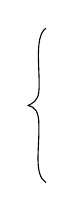
\begin{tikzpicture}[x=.45cm,y=.7cm]
\draw (0,1.4) .. controls (-.35,1.25) and (-.15,.6) .. (-.2,.25)
.. controls (-.22,.08) and (-.4,.03) .. (-.5,0)
.. controls (-.3,-.03) and (-.2,-.12) .. (-.2,-.35)
.. controls (-.18,-.8) and (-.35,-1.25) .. (0,-1.4);
\end{tikzpicture}}}
(ii) Si \deleted{$\unsure{g}\!:\!Y$}
\diagram{\begin{tikzcd}
Y\arrow[r,"i"]\arrow[d,"{\deleted{\unsure{g}}\,f}"']&X\arrow[d,dash,"g"]\\
Y'\arrow[r,dash]&X'
\end{tikzcd}}
cocartésien, avec $i,f\in\unsure{\mathcal M|\mathcal A}$, et $f\in\underline W$, alors $g\in W$.

(iii) $\exists$ familles génératrices d'intervalles les $I_\alpha$, telles que pour
$\forall X$, $X\amalg X\longrightarrow X\times I_\alpha$ soit $\in\unsure{\mathcal M|\mathcal A}$.
\margin{Ce sont donc des intervalles séparants}

\margin{$\Vert$}
(\unsure{iv|0}) $\varinjlim$ finies existent dans $\underline M$, et \deleted{les}
\deleted{sommes \inserted{\uline{directes}} \unsure{dans} $\in\unsure{W}$},
$f,g\in W\ \Longrightarrow\ f\amalg g\in W$.

\margin{\diagram{\begin{tikzcd}&{}\arrow[dl]\\{}&\end{tikzcd}}}
\margin{L'énoncé des conditions (i) à (iv) \unsure{s'inspire du cas de}
$(\mathrm{Cat})$ et non celui de $\widehat A$, où (iii) est inutile,
pourvu que dans (ii) il suffise \unsure{d'imposer} $i$ (ou $f$) $\in\underline W$.}

\margin{Dans tout $(M,W)$ \unsure{pourvu d'une} \deleted{\unsure{structure}}
$h$ (compatible à $W$ [car les homotopismes sont dans $W$])
$W^{-1}M=\overline W^{-1}\overline M$, et $\overline W$ admet un calcul de fractions
à gauche, moyennant les conditions (i) à (iv) :}
\margin{\deleted{\unsure{modifier pour les cas généraux}}}

\margin{\unsure{Giordano Br}}

\scanpage{26}
\mspage{7}
% archive foliation: 25
\margin{\deleted{\uline{\unsure{Foutaise}}}}

Dans cet argument, il a fallu \inserted{\unsure{visiblement}} utiliser un intervalle
$I$ \uline{séparant} (cf condition (iii)). Donc dans le cas $M=\widehat A$, il faut
disposer d'un intervalle $I$ \uline{séparant} dans $\widehat A$
\deleted{dans $A$} qui de plus définisse une \deleted{\unsure{théorie}}\inserted{structure}
homotopique sur $\widehat A$ \deleted{\unsure{pour}}\inserted{compatible} avec $W$
--- et pour ceci, il faut supposer que
$I\longrightarrow e$ est $\underline W_A$-asphérique
[ou du moins que \deleted{les deux extrémités}\inserted{$\delta_0$ et $\delta_1:e\longrightarrow I$}
\deleted{\unsure{aient}} \uuline{$\mathrm{univ}^{t}$}
$\Rightarrow$ image dans $W$ $\ldots$] --- donc, finalement, que
\deleted{\unsure{donc}} \margin{$\Vert$} $A$ soit une catégorie-test \uline{locale}.
\margin{\uline{NB} \unsure{c'est inutile}, \unsure{cf ci. $h$}
\unsure{Si on regarde la catégorie $A$} \deleted{\unsure{puisque}}}
\margin{\deleted{\unsure{doit être} \unsure{une catégorie} \unsure{test}}}

On a utilisé aussi la propriété (pour \unsure{cas} $J=2$) que pour une famille de
flèches $(f_j)_{j\in J}$ dans $\widehat A$, $f_j\in\underline W_A$ pour
$\forall j\in J\ \Longrightarrow\ \coprod_j f_j\in\underline W_A$.
On est ramené à voir la $=$ chose dans $(\mathrm{Cat})$, pour $\underline W$.
Cela résulte alors de loc. 3 (condition de \unsure{localis.tion}) appliqué à
\diagram{\begin{tikzcd}
X\arrow[r]\arrow[dr]&Y\arrow[d]\\&J
\end{tikzcd}}.

\deleted{Coroll.}

\scanpage{27}
% archive foliation: 26
\uline{Corollaire 1} Dans $\mathrm{Hot}(\underline W)$, les sommes directes finies existent, et les foncteurs canoniques $(\mathrm{Cat})\longrightarrow\mathrm{Hot}(\underline W)$, $\widehat A\longrightarrow\mathrm{Hot}_A,\longrightarrow\mathrm{Hot}(\underline W)$ y commutent.

\margin{\uline{finies} inutile, \unsure{par argument plus bas}}
\margin{pas de conditions sur $A$ ici! \diagram{\begin{tikzcd}&{}\\{}\arrow[ur]&\end{tikzcd}}}

On est ramené au cas de $(\mathrm{Cat})$ (vu que $i_A:\widehat A\longrightarrow(\mathrm{Cat})$ commute aux $\varinjlim$ \unsure{donc aux} sommes), via le

\margin{$|$}\uline{Lemme} Soit $(\underline M,W)$ avec $W\subset\mathrm{Fl}(\underline M)$, $W$ permettant calcul des fractions à droite. \deleted{Si dans $M$ les} \inserted{Alors} \inserted{le} foncteur canonique $M\longrightarrow W^{-1}M$ commute aux $\varinjlim$ finies, \deleted{\unsure{les}} et en particulier aux sommes finies.

On appliquera ceci à $(\overline{\mathrm{Cat}},\overline{\underline W})$, il faut voir que les sommes finies y existent (sinon le lemme n'apprend pas \unsure{gd} chose!), et que $\mathrm{Cat}\longrightarrow\overline{\mathrm{Cat}}$ y commute. \deleted{Donc} Mais on a de façon générale

\scanpage{28}
% archive foliation: 27
\uline{Lemme} \unsure{Soit} $(M,h)$ structure homotopique par intervalles (homotopy interval structure), avec $M$ stable par sommes [finies], et les sommes [finies] étant universelles. Alors $M\longrightarrow W_h^{-1}M$ commute aux sommes finies.

\margin{\uline{NB} $M$ stable par produits finis}

Cela revient à ceci: pour
\diagram{\begin{tikzcd}[column sep=large]
\begin{gathered}f=(f_j)_{j\in J}:\\g=(g_j)_{j\in J}\end{gathered}
& \underbrace{\coprod_J X_j}_{X}\arrow[r,shift left=.5ex,"f"]\arrow[r,shift right=.5ex,"g"'] &Y
\end{tikzcd}}
\margin{$\vert$}
\[
f\underset h\sim g\quad\unsure{\text{ssi}|\text{sss}}\quad f_j\underset h\sim g_j\quad\forall j\in J.
\]
\uline{Dém} $\Rightarrow$ trivial, pour prouver $\Leftarrow$ on note qu'il existe \uline{un $\unsure{=}$ intervalle} $I$ tel que $f_j\underset{h_I}\sim g_j$ \deleted{$\unsure{(I\subset)}$} (car $J$ est fini), \deleted{on prend} comme
\[
I\times X=\coprod_J I\times X_j
\]
on trouve homotopie composée
\deleted{$\unsure{I\times}$}
\diagram{\begin{tikzcd}[column sep=large,row sep=small]
I_N\times X\arrow[r]&X\\
\cup&\cup\\
I_N\times X_j\arrow[r]&X_j
\end{tikzcd}}
(avec $N$ assez grand pour convenir pour tous les $j$\ldots). On gagne!

\scanpage{29}
% archive foliation: 28
\uline{NB} Il semble \uline{faux} que $(\mathrm{Cat})\longrightarrow\overline{\mathrm{Cat}}$ commute aux sommes infinies --- Il suffit de prendre \deleted{de} \unsure{une} \unsure{foule|famille}
\diagram{\begin{tikzcd}[column sep=large]
\begin{gathered}f_n\\g_n\end{gathered} & X_n\arrow[r,shift left=.5ex]\arrow[r,shift right=.5ex]&Y
\end{tikzcd}}
$(n\in\mathbb N)$ telles que $f_n\underset{\unsure{h}}\sim g_n$, mais qu'il faut une suite d'au moins $n$ homotopies él. pour les joindre (prendre p.ex. $X_n=\Delta_0$, $f_n,g_n$ définis par des pts de $Y$, prendre
\[
Y=I_\infty=(
\]
\diagram{\begin{tikzcd}[column sep=small]
{}\arrow[r]\arrow[rr,phantom,"\underbrace{\hspace{1.35cm}}"'] & {} & {}\arrow[l]\arrow[r]\arrow[rr,phantom,"\underbrace{\hspace{1.35cm}}"'] & {} & {}\arrow[l] & \cdots
\end{tikzcd}}
somme amalgamée d'une infinité de copies de $X_n$, \deleted{Mais} \deleted{\unsure{je soup}} la somme $\coprod X_n$ \uline{n'est pas} une somme dans $\overline{\mathrm{Cat}}$, car Je soupçonne pourtant que dans $\mathrm{Hot}(\underline W)$, les sommes quelconques existent et que $\mathrm{Cat}\longrightarrow\mathrm{Hot}(\underline W)$ y commute??

\margin{\unsure{Jobs au Trave|Jobs au Travail}}

\scanpage{30}
% archive foliation: 29
\margin{\unsure{Copies pédagogiques}\\\unsure{Matériau}}
\deleted{Pourtant, soit $X$}

Il revient au $=$ de dire que pour $(X_j)_{j\in J}$ et $Y$ dans $(\mathrm{Cat})$, si \inserted{$X=\coprod X_j$}
\[
\operatorname{Hom}_{\mathrm{Hot}}(\deleted{\unsure{\Phi}(}X),\deleted{\unsure{\Phi}(}Y))\longrightarrow\prod_{j\in J}\operatorname{Hom}_{\mathrm{Hot}}(X_j,Y)
\]
est bijectif. Mais avec le calcul des fractions, ni l'i\deleted{\unsure{bije}}\unsure{n}jectivité ni la surjectivité n'est claire, elles auraient l'air plutôt fausses, pour les $=$ raisons. C'est quand $=$ bien gênant! \deleted{\unsure{?}}

$a)$ Il se pourrait que pour des \deleted{\unsure{Dém}} éléments des seconds $\unsure{\mathrm m^{\mathrm b}|=^{\mathrm b}}$ $(\varphi_j)_{j\in J}$, il n'existe pas de $(Y\longrightarrow Y')\in W$ \uline{commun pour tous les} $\varphi_j$, tels que
\diagram{\begin{tikzcd}[column sep=large]
X_j\arrow[r,dashed,"\varphi_j"]&Y
\end{tikzcd}}
se représente par
\diagram{\begin{tikzcd}
X_j\arrow[r,"f_j"]&Y'
\end{tikzcd}}
À priori, on aura $Y\lhook\joinrel\longrightarrow Y'_j$ (imm. fermée si on veut), mais \unsure{quand} $=$ par le \unsure{thm.} des \unsure{passages}: les limites, prises par parties finies

\scanpage{31}
% archive foliation: 30
$J_0$ de $J$
\[
Y'_{J_0}=\coprod_{j\in J_0}\!{}_Y\,\unsure{Y'_{J_0}|Y'_j},
\]
et $Y'_J=\varinjlim Y'_{J_0}$, on aura $Y\longrightarrow Y'\in\underline W$. Donc il y aura quand $=$ surjectivité! Mais soient maintenant
\diagram{\begin{tikzcd}[column sep=large]
f,g:X\arrow[r,shift left=.5ex,"\unsure{f_0|f}"]\arrow[r,shift right=.5ex,"g"']&\deleted{Y'}\inserted{Y}
\end{tikzcd}}
qui \deleted{\unsure{deviennent}} sont tels que $\unsure{\sigma|\gamma}(f_j)=\unsure{\sigma|\gamma}(g_j)$ $\forall j\in J$, a-t-on $\unsure{\sigma|\gamma}(f)=\unsure{\sigma|\gamma}(g)$? Mais oui, par le $=$ argument --- condensé dans un

\margin{\uuline{bof!}}

\uline{Lemme} Soit $Y\xrightarrow{\alpha_j}Y'_j$ \deleted{de} une \unsure{foule|famille} d'équivs. faibles, alors il existe $Y\xrightarrow{\alpha}Y'$ une équiv. faible \deleted{telle que} \inserted{$Y\lhook\joinrel\longrightarrow Y'$} (imm. ouverte ou fermée si on y tient) \deleted{telle que} des $\beta_j:Y'_j\longrightarrow Y'$ tels que $\beta_j\alpha_j=\alpha$.

\margin{\diagram{\begin{tikzcd}[column sep=large,row sep=large]
Y\arrow[r,hook,"\bar\alpha_j"]\arrow[dr,"\alpha"']&\overline{Y'_j}\arrow[r,shift left=.5ex,"i_j"]\arrow[d]&Y'_j\arrow[l,dashed,shift left=.5ex,"r_j"]\arrow[dl,dashed,"\beta_j"]\\
&Y'&
\arrow[from=1-1,to=2-2,phantom,"\mathrm{comm}"{pos=.55}]
\arrow[from=1-3,to=2-2,phantom,"\mathrm{comm}"'{pos=.6}]
\end{tikzcd}}
$r_ji_j=\mathrm{id}_{\overline{Y'_j}}$}

(De plus, si les $\alpha_j$ sont des imm. ouvertes, resp. fermées, on peut prendre pour $Y'$ la somme amalgamée des $Y'_j$.)

On est ramené à prouver ceci: Soient $f,g:X=\coprod X_j\longrightarrow Y$, tels que $f_j\sim g_j$ $\forall j\in J$, alors $\unsure{\sigma|\gamma}(f)=\unsure{\sigma|\gamma}(g)$. (Mais attention on n'aura pas $f\sim g$!) \uline{Il faut une condition du type ``\unsure{Kan}'' sur $Y$}, ou plutôt un $Y'$, où $(Y\longrightarrow Y')\in\underline W$.

\scanpage{32}
% archive foliation: 31
\uline{Corollaire 2} \uline{Dans} $\mathrm{Hot}(\underline W)$, les produits finis existent, et les foncteurs canoniques $(\mathrm{Cat})\longrightarrow\mathrm{Hot}(\underline W)$, $\widehat A\longrightarrow\mathrm{Hot}(\underline W)$ ($A$ catégorie test stricte) y commutent.

\margin{\diagram{\begin{tikzcd}[column sep=small,row sep=small]
{}\arrow[dr]&\\&{}
\end{tikzcd}}il suffit $=$ que $A$ soit tot. $\underline W$-asph.}

On est ramené à prouver que
\[
\widehat A\longrightarrow[\mathrm{Hot}(\underline W)\simeq]\underline W_A^{-1}\widehat A
\]
commute aux produits finis, i.e. que
\[
(*)\quad\operatorname{Hom}_{\underline W_A^{-1}\widehat A}(X,\unsure{Y_j|Y})\longrightarrow\prod_J\operatorname{Hom}_{\underline W_A^{-1}\widehat A}(X,Y_j)
\]
est bijectif, pour \unsure{tte} famille finie $(Y_j)_{j\in J}$ d'objets de $\widehat A$, et $X$ de $\widehat A$.

\margin{\deleted{\unsure{on voit}} Mais le cas de $(\mathrm{Cat})$ se traite directement.}

\uline{Surjectivité} Un élément du $2^{\mathrm o}$ \unsure{mb} provient d'une famille
\diagram{\begin{tikzcd}
f_j:X\arrow[r]&Y'_j
\end{tikzcd}}
où $Y_j\longrightarrow Y'_j$ équiv. faible.

\deleted{\uline{\unsure{Dém}}}\inserted{Considérons} alors
\[
f=(f_j):X\longrightarrow\prod Y'_j=Y'
\]
il définit $X\longrightarrow Y$ qui convient, \uline{si on sait que} $\prod Y_j\longrightarrow\prod Y'_j$ est $\in\underline W$.

\scanpage{33}
% archive foliation: 32
C'est le cas si $A$ catégorie test stricte, plus \unsure{génlt} si elle est \unsure{tot.} $\underline W$-asphérique.

\uline{Lemme} \unsure{(!)|(?)} Soit $A$ \deleted{une catégorie \unsure{finie}} \inserted{dans $(\mathrm{Cat})$}. \inserted{Conditions équiv.}

$(i)$ $A$ \deleted{est} tot. $\underline W$-asphérique, \deleted{il faut}

$(ii)$ \deleted{que produit de $2$ flèches $(\underline W_A)$}\inserted{Produit fini de flèches $(\underline W_A)$} est $\in\underline W_A$

\deleted{$\unsure{(iii)}$}\inserted{$(ii\ \mathrm{bis})$} Si $f:X\longrightarrow Y$ \deleted{dans $A$} est dans $\underline W_A$ et $Z$ dans $\widehat A$, $f\times\mathrm{id}_Z:X\times Z\longrightarrow Y\times Z$ est dans $\underline W_A$

$(iii)$ Le foncteur $\widehat A\longrightarrow(\mathrm{Hot}_A(\unsure{\underline W}))$ commute aux produits finis
\deleted{\uline{Dém}}

$(iv)$ Le foncteur $\widehat A\longrightarrow(\mathrm{Hot}_{\unsure{A}}(\underline W))$ commute aux produits finis

\margin{\diagram{\begin{tikzcd}[row sep=large,column sep=huge]
(i)\arrow[d,Rightarrow]\\
(ii)\arrow[d,Leftrightarrow]\\
(ii\ \mathrm{bis})\arrow[d,Rightarrow]\arrow[uu,Rightarrow,bend left=65,"{[\text{si }A\ \deleted{\unsure{est}}\ \underline W\text{-asph.}]}"']\\
(iii)\arrow[u,Rightarrow,bend left=65,"\text{\unsure{si: saturation forte|si: résolution forte}}"']
\end{tikzcd}}
\deleted{\unsure{cat. test faible}}}

On va revenir à ce lemme tantôt. Pour le moment, on suppose vérifié $(ii)$, qui assure surjectivité de $*$.

\uline{Injectivité}?
\diagram{\begin{tikzcd}[column sep=large,row sep=large]
&Y\arrow[d,"\alpha"',"\in W"]\arrow[r,"\mathrm{pr}_j"]&Y_j\arrow[d,"\beta_j"',"\in\underline W"]\\
f,g:X\arrow[r,shift left=.5ex]\arrow[r,shift right=.5ex]&Y'\arrow[r,"\varphi_j"']&Y'_j\deleted{{}=\unsure{Y'\amalg_Y Y_j}}
\end{tikzcd}}
on suppose que pour $\forall j$, $\exists\,\beta_j:Y_j\longrightarrow Y'_j$, $\varphi_j$ tels que $\beta_j\mathrm{pr}_j=\varphi_j\alpha$, $\beta_j\in\underline W$, $\varphi_jf\underset h\sim\varphi_jg$,
\deleted{Donc}\deleted{On a donc}\deleted{\unsure{?}} posons
\[
\beta=\prod\beta_j:Y=\prod Y_j\longrightarrow Y''=\prod Y'_j,
\]
\deleted{\unsure{pourra}} on trouve

\scanpage{34}
% archive foliation: 33
diag. commutatif
\diagram{\begin{tikzcd}[column sep=large,row sep=large]
&Y\arrow[d,"\alpha\in W"']\arrow[dr,dash,"\beta=\prod\beta_j\in W"]&\\
X\arrow[r,shift left=.6ex,"f"]\arrow[r,shift right=.6ex,"g"']&Y'\arrow[r,"\varphi=(\varphi_j)"']&Y''=\prod Y'_j
\arrow[from=1-2,to=2-3,phantom,"\mathrm{comm}"'{pos=.55}]
\end{tikzcd}}
avec $\varphi f\sim\varphi g$, donc $\unsure{\sigma|\gamma}(f)=\unsure{\sigma|\gamma}(g)$

\uline{NB} Cela marcherait pour les produits infinis, si on savait qu'un produit infini d'éléments de $\underline W_A$ est encore dans $\underline W_A$

Venons-en au lemme plus haut
\[
(ii)\Longleftrightarrow(ii\ \mathrm{bis})\quad\text{trivial}
\]
($\Longleftrightarrow$ si $f\in\underline W_A$, alors $\forall a\in\operatorname{Ob}A$, $f\times\mathrm{id}_a:X\times a\longrightarrow Y\times a$ \inserted{$\in\underline W_A$})
\diagram{\begin{tikzcd}[row sep=large]
{}\arrow[d,Rightarrow,"\text{on vient de le prouver}"]\\(iii)
\end{tikzcd}}
\margin{\diagram{\begin{tikzcd}{}\\(iii)\arrow[u,Rightarrow]\end{tikzcd}}
est évident quand on sait que $\underline W_A$ est fortement saturé (\unsure{résulte de} $\unsure{\underline W}$ fortement saturé)}

\deleted{Examinons $(iii)$}

$(ii\ \mathrm{bis})$ \deleted{signifie} aussi que si $f\in\underline W_A$, alors $\forall Z$, $f\times\unsure{\mathrm{id}}_Z:X\times Z\longrightarrow Y\times Z$ est $\in\underline W_A$ loc. sur $Z$, et pour ceci il suffit de le voir pour $Z$ dans $A$, i.e.

\margin{raisonnement déjà fait plus haut}
\diagram{\begin{tikzcd}[column sep=large,row sep=large]
X\times a\arrow[r,"\in W"]\arrow[d]&Y\times a\arrow[d,dash]\\
X\arrow[r,"\in\underline W_A"']&Y
\end{tikzcd}}
Cela marche si on sait que $X\times a\longrightarrow X$ \inserted{et $Y\times a\longrightarrow Y$} $\in\underline W_A$, ce qui signifie aussi que $\unsure{\widehat A|A}$ est tot. asph. \deleted{et} Donc $(i)\Longrightarrow(ii\ \mathrm{bis})$

\deleted{En fait}\deleted{de même $(ii\ \mathrm{bis})$ implique} Inversement, on voit tout de suite que si $A$ asph, alors $(ii\ \mathrm{bis})\Longrightarrow(i)$ [prendre $f:a\longrightarrow e_{\widehat A}$)
\inserted{donc $(i)\Longleftrightarrow(\unsure{(ii)|(iii)}+A$ asphérique}

\scanpage{35}
% archive foliation: 34
Reste à examiner $(iv)$. Comme on sait déjà que $(\mathrm{Cat})\longrightarrow\mathrm{Hot}(\underline W)$ commute aux produits finis, $(iv)$ signifie que pour $X,Y$ dans $\widehat A$,
\deleted{$\unsure{A_{/X}\times A_{/Y}}$}
\[
A_{/X\times Y}\longrightarrow A_{/X}\times A_{/Y}
\]
est $\in\underline W$. \deleted{Cela implique} Dans le cas $X=a$, $Y=b$ dans $\operatorname{Ob}A$, cela signifie que $a\times b$ asphérique --- i.e. $\widehat A$ tot. \inserted{$\underline W$-}asph. Je dis que cela suffit, de façon précise que $A_{/X\times Y}\longrightarrow A_{/X}\times A_{/Y}$ est asph.

En effet, pour un objet $\alpha=(a_{/x},b_{/y})$ du deuxième \unsure{mb}, on a
\[
(A_{/X\times Y})_{/\alpha}\simeq A_{/a\times b}
\]
\deleted{et} on gagne. En résumé

\diagram{\begin{tikzcd}[column sep=large,row sep=large,execute at end picture={
\coordinate (bracetop) at ([xshift=-1em]\tikzcdmatrixname-1-2.west);
\coordinate (bracemid) at (bracetop |- \tikzcdmatrixname-2-2.west);
\coordinate (bracebot) at (bracetop |- \tikzcdmatrixname-3-2.west);
\draw (bracetop) .. controls ([xshift=-.4em,yshift=-.5em]bracetop) and ([xshift=.2em,yshift=.5em]bracemid) .. ([xshift=-.4em]bracemid) .. controls ([xshift=.2em,yshift=-.5em]bracemid) and ([xshift=-.4em,yshift=.5em]bracebot) .. (bracebot);
\coordinate (bracetwotop) at ([xshift=-1em]\tikzcdmatrixname-4-2.west);
\coordinate (bracetwobot) at (bracetwotop |- \tikzcdmatrixname-5-2.west);
\path (bracetwotop)--(bracetwobot) coordinate[pos=.5] (bracetwomid);
\draw (bracetwotop) .. controls ([xshift=-.4em,yshift=-.3em]bracetwotop) and ([xshift=.2em,yshift=.3em]bracetwomid) .. ([xshift=-.4em]bracetwomid) .. controls ([xshift=.2em,yshift=-.3em]bracetwomid) and ([xshift=-.4em,yshift=.3em]bracetwobot) .. (bracetwobot);
}]
& (i)\quad A\text{ tot. }\underline W\text{-asph.}\arrow[d,Leftrightarrow]\\
\left.\begin{gathered}a\longrightarrow X\times Y\\a\longrightarrow X\\a\longrightarrow Y\end{gathered}\right\}\arrow[r,"a"]
&(iv)\quad\widehat A\longrightarrow\mathrm{Hot}(\underline W)\text{ commute aux produits binaires}\arrow[d,Leftrightarrow]\\
&(iv\ \mathrm{bis})\quad\widehat A\longrightarrow\mathrm{Hot}(\underline W)\text{ commute aux produits finis}\arrow[d,Rightarrow]\\
&(ii)\quad\deleted{\unsure{Produit}}\inserted{\underline W_A\text{ stable}}\text{ par produits finis}\arrow[d,Leftrightarrow]\arrow[u,Rightarrow,bend left=70,"\text{si }A\ \underline W\text{-asph.}"']\\
&(ii\ \mathrm{bis})\quad f\in\underline W_A\Longrightarrow f\times\mathrm{id}_X\in\underline W_A\quad(\forall X\in\operatorname{Ob}\widehat A)\arrow[d,Rightarrow]\\
&(iii)\quad\widehat A\longrightarrow\mathrm{Hot}_A\text{ commute aux produits finis}\arrow[u,Rightarrow,bend left=65,"\text{\unsure{forte saturation}}"']
\end{tikzcd}}

\scanpage{36}
% archive foliation: 35
\deleted{Mais il n'est pas clair pour moi si}

\deleted{la} \uline{NB} La condition $(ii)$ est visiblement stable par sommes (i.e. si des $A_\alpha$ y satisfont, $A=\coprod_\alpha A_\alpha$ aussi), mais la condition $(i)$ non, donc \deleted{$(i)$ est} \inserted{l'implication} $(i)\Longrightarrow(ii)$ est stricte. Mais un $A$ qui satisfait $(ii)$, et qui est $0$-connexe \deleted{\unsure{je}} est alors \inserted{$\underline W$-}asphérique (même tot. $\underline W$-asphérique).

\uuline{NB} Prenons p.ex. \deleted{un} $A$ un groupoïde, alors dans $\widehat A$ $\underline W_A$ est formé des seuls iso (cas où $\underline W$ est l'équiv. faible habituelle) donc stable \uline{par produits} finis...

Cet argument de commutation \inserted{aux produits finis} marche directement dans $(\mathrm{Cat})$ également, \deleted{\unsure{donc on sait}} \inserted{puisqu'on sait} qu'un produit \deleted{\unsure{cartésien}} fini de foncteurs $\in\underline W$ est $\in\underline W$.

Pour le cas des produits infinis, il faut voir qu'un produit des $f_j\in\underline W$ est dans $\underline W$, \deleted{et} et/ou item dans un $\widehat A$ (le deuxième impliquera le premier). Déjà pour l'équiv. faible habituelle $\underline W_0$, ce n'est pas évident. Il y a des

\scanpage{37}
% archive foliation: 36
chances qu'on arrive à le ramener à prouver qu'un produit $\prod_{j\in J}X_j$ d'\unsure{espaces} $\underline W$-asphériques est $\underline W$-asphérique? Ça me semble moins important de toutes façons que la question des sommes infinies.

\margin{Ahmed}

\scanpage{39}
% archive foliation: 38
Passage à la limite

\uline{\unsure{Thm}} Soient $I$ un ordonné \deleted{filtrant}, $X,Y$ dans $(\mathrm{Cat})$, $(X_i)_{i\in I}$ et $Y=(Y_i)_{i\in I}$ deux filtrations par des sous-cat. fermées (resp. ouvertes), \deleted{\unsure{$f$}} $X=\bigcup X_i$, $Y=\bigcup Y_i$.
\[
f:X\longrightarrow Y
\]
tel que $f(X_i)\subset Y_i$, soit $f_i:X_i\unsure{\mathbin{-}|\longrightarrow}Y_i$.
Supposons que les $f_i$ soient des équiv. faibles, alors $f$ est une équiv. faible.

\margin{\unsure{On suppose que les inf existent et que les filtrations} \unsure{commutent}, \unsure{dans le cas où} $i=\operatorname{Inf}j_\alpha$, \unsure{on ait} $X_i=\bigcap_\alpha X_{j_\alpha}$.}

On est ramené par dualité au cas des ss-catégories ouvertes. On va \deleted{\unsure{supposer}} interpréter la filtration de $X$ comme la donnée de
\diagram{\begin{tikzcd}X\arrow[r,"\varphi"]&I\end{tikzcd}}
défini par
\[
\varphi(x)=\operatorname{Inf}_{\substack{i\text{ dans }I(x)=\\\{i\in I\mid x\in X_i\}}}i
\]
--- on suppose donc que dans $I$ les Inf \inserted{(des parties non vides)} existent. On \deleted{\unsure{pourra}} \inserted{aura}, pour
\[
\alpha:x\longrightarrow y
\]
$\varphi(x)\leq\varphi(y)$ (car $I(y)\subset I(x)$, donc $\operatorname{Inf}I(y)\geq\operatorname{Inf}I(x)$) d'où la valeur de $\varphi(\alpha)$. On \deleted{\unsure{aura supposé, où}} \inserted{devra supposer}
\[
X_i=\varphi^{-1}(I_i)\qquad\text{où}\qquad I_i=\{j\in I\mid j\leq i\}
\]
\deleted{\unsure{$\varphi$}} i.e. $\underbrace{x\in X_i}_{\text{i.e. }i\in I(x)}\Longleftrightarrow\varphi(x)\leq i$

\margin{\uline{NB} $\varphi(x)$ est ainsi le plus petit élément de $I(x)$ et $I(x)=\{j\in I\mid j\geq\varphi(x)\}$.}

\scanpage{40}
% archive foliation: 39
\deleted{Bien sûr, par définition,}

\uline{Il \unsure{faudr.} expliciter} que pour une catégorie $I$ d'indices, telle que les Inf des parties non vides existent, les foncteurs $X\longrightarrow I$ sont en corr. $1$-$1$ avec les filtrations \deleted{\unsure{croiss.}} applications croissantes
\[
\begin{aligned}I&\longrightarrow\operatorname{SsCatOuv}(X)\\i&\longmapsto X_i\end{aligned}
\]
qui commutent aux dits Inf, et telles que l'on ait $X=\bigcup X_i$.
\margin{cette dernière condition équivaut aussi à $\varinjlim X_i\simeq X$.}

Ceci posé, on a
\[
X_{/i}=X_i
\]
\deleted{d'où \unsure{l'explicitation}, pour $f$}
\[
f_i:X_i\mathbin{-}Y_i
\]
s'identifie à
\[
f_{/i}:X_{/i}\mathbin{-}Y_{/i}
\]
donc on gagne par L3.

\margin{$\vert$}
\uline{Corollaire \unsure{1|!}} Idem dans un $\widehat A$, en utilisant le fait que $i_A$ commute aux \uline{$\varinjlim$} quelconques et \deleted{aux} produits fibrés.

\margin{\uline{Cor?} Si les $X_i$ sont \inserted{$\underline W$-}asphériques et $I$ connexe, alors $X$ est $\underline W$-asphérique (On prend $Y_i=\unsure{e_{(I_i)}|e_i}$).}

\uuline{Thm} L'ens. $\underline W$ est saturé

\uline{Cor} Pour $\forall A$, $\underline W_A$ est saturé.

\deleted{
\uline{Dém} Soit $f:X\mathbin{-}Y$ tel que $\unsure{\sigma|\gamma}(f)$ iso, d'où
\diagram{\begin{tikzcd}[column sep=small,row sep=small]
X\arrow[dr,"f"]&&X\arrow[d,"\alpha\in\underline W"']\arrow[drr,"f"]\\
&Y\arrow[r,"g"]\arrow[l,phantom,"\unsure{\exists}"]&X'\arrow[drr,"f'"']&&Y\arrow[d,"\beta\in\underline W"]\\
&&&&Y'
\end{tikzcd}}
\deleted{avec $\unsure{\sigma|\gamma}(gf)=\unsure{\sigma|\gamma}(\alpha)$, et}
avec $\unsure{\sigma|\gamma}(gf)=\unsure{\sigma|\gamma}(\alpha)$, $\unsure{\sigma|\gamma}(f'g)=\unsure{\sigma|\gamma}(\beta)$, $\beta f\simeq f'\alpha$.

Quitte à changer $\alpha$ en composé avec $X'\mathbin{-}X'_1$, et item pour $Y'$ avec $Y'\mathbin{-}Y'_1$, OPS $gf\sim\alpha$, $f'g\sim\beta$, \inserted{donc $gf\in\underline W$, $f'g\in\underline W$} \deleted{et pr (quitte à changer encore $\alpha$ et $\beta$ par $gf$ et $f'g$) \unsure{qui sont égales}}
\diagram{\begin{tikzcd}
X\arrow[r,"f"]\arrow[d,"\alpha"']&Y\arrow[d,"\beta"]\arrow[dl,"g"']\\
X'\arrow[r,"f'"']&Y'
\end{tikzcd}}
\[
\underbrace{\begin{gathered}\alpha,\beta\in W\\gf=\alpha,\quad f'g=\beta\\(\text{quitte à \unsure{factoriser}})\end{gathered}}
\]
\margin{\diagram{\begin{tikzcd}[column sep=small]
X\arrow[r,"f"']&Y\arrow[r,"g"']&Y'\arrow[r,"f'"']&X'
\end{tikzcd}} $gf\in\underline W$, $f'g\in\underline W$}

On pourrait d'ailleurs supposer que $f$ soit imm. ouverte, puis (quitte à factoriser \deleted{$g$, puis $f'$}) que $f,g,f'$ \unsure{sont|soient} des imm. ouvertes.
\unsure{\diagram{\begin{tikzcd}[row sep=large,column sep=large]
X\arrow[rr,hook]&&Y\arrow[dl,"g_1"']\\
&X'_1\arrow[dl,shift right]\arrow[dr,hook]\\
X'\arrow[ur,shift right]\arrow[rr]&&Y'
\end{tikzcd}}}
}

\scanpage{41}
% archive foliation: 40
Soit $f=f_0\in\operatorname{Fl}(\unsure{\underline{\mathrm{Cat}}|\mathrm{Cat}})$ \inserted{:\unsure{$f$}$:X_0\mathbin{-}X_1$} telle que $\unsure{\sigma|\gamma}(f)$ iso: prouver $f\in\underline W$. OPS $f=f_0$ imm. ouverte. Par calcul des fractions, $\exists\unsure{f_1|g}:X_1\mathbin{-}X_2$, telle que $\unsure{f_1|g}f_0\in\underline W$; donc $\unsure{\sigma|\gamma}(\unsure{f_1|g}f_0)=\unsure{\sigma|\gamma}(\unsure{f_1|g})\unsure{\sigma|\gamma}(f_0)$ iso, donc $\unsure{\sigma|\gamma}(\unsure{f_1|g})$ iso. OPS quitte à factoriser que $g$ imm. ouverte.

\margin{\diagram{\begin{tikzcd}[row sep=tiny,column sep=large]
X_0\arrow[d,equal]&X_1\arrow[d,equal]\\
X\arrow[r,"\substack{f\\\Vert\\f_0}"']&Y\arrow[r,dash,"\substack{g\\\Vert\\f_1}"']&X_2
\end{tikzcd}}}

Donc de proche en proche
\deleted{$f_0,g_0,f_1,g_1,\unsure{f_n|f_2},\unsure{g_n|g_2}$}
\deleted{$f_0,f_1,f_2$}
\deleted{donc}
\diagram{\begin{tikzcd}[column sep=large]
X_0\arrow[r,"f_0=\unsure{f}"]&X_1\arrow[r,"f_1=\unsure{g}"]&X_2\arrow[r,dash,"\unsure{f_3|f_2}"]&{}
\end{tikzcd}}
système inductif d'imm. ouvertes, telles que les produits de deux consécutifs \unsure{soit|soient} $\in\underline W$. Soit $X_\infty=\varinjlim_n X_n$, on a
\diagram{\begin{tikzcd}
X_0\arrow[rr,"f=f_0"]\arrow[dr,"i_0"']&&X_1\arrow[dl,"i_1"]\\
&X_\infty&\text{commutatif}
\end{tikzcd}}
il suffit de prouver que $i_0$ et $i_1$ sont $\in\underline W$.
\deleted{\unsure{Cela résulte du}} \inserted{Il suffit bien sûr de} le prouver pour $i_0$ \deleted{\uline{\unsure{lemme}}} [pour $i_1$, on remplacera $f_0$ par $f_1$]. Or on a
\diagram{\begin{tikzcd}[column sep=small,row sep=large]
X_0=\varinjlim_n\arrow[d,"i_0"']&(&X_0\arrow[r,dash]&X_0\arrow[r,dash]&X_0\arrow[r]&\cdots&X_0\unsure{)}\arrow[d]\arrow[r,dash]&\cdots&)\\
X_\infty=\varinjlim_n&(&X_0\arrow[r,dash]&X_2\arrow[r,dash]&X_4\arrow[r,dash]&\cdots&X_{2n}\arrow[r,dash]&\cdots&)
\end{tikzcd}}
et $i_0$ est $\varinjlim$ des $i_0^{2n}:X_0\mathbin{-}X_{2n}$, qui sont $\in\underline W$: donc on gagne!!

\margin{\deleted{\unsure{Djamel|Djamal}}}
